\chapter{Specific Requirements}
\label{chap:specific-requirements}%

\par This chapter provides detailed specifications for the requirements previously mentioned that may require
additional clarification for the development team's implementation.

\section{External Interface Requirements}
\label{sec:external-interface-requirements}%

\subsection{User Interfaces}
\label{subsec:user-interfaces}%

\par The user interface of S\&C is implemented as a web-based application, making it accessible through standard web
browsers. No specialized software installation is required - users only need a web browser and an internet connection
to access all platform features.

\subsection{Hardware Interfaces}
\label{subsec:hardware-interfaces}%

\par S\&C – being a web application – will be available on all devices, connected to the internet, capable of running a
modern browser. Users can use S\&C on laptops, desktops, smartphones, tablets, ...

\subsection{Software Interfaces}
\label{subsec:software-interfaces}%

\par The system will primarily function as a standalone application. The only external dependency is the SSO portals of
the various UN organizations that have requested enrollment in S\&C, which will provide access to UN personnel and STs.

\subsection{Communication Interfaces}
\label{subsec:communication-interfaces}%

\par The system primarily relies on HTTPS for secure communication. This includes communication between users and the
frontend, as well as between the frontend and backend, and between the backend and the various SSO portals.

\par The SMTP protocol is also used to send notifications to the user's email address when necessary.

\section{Functional Requirements}
\label{sec:functional-requirements}%

\subsection{Requirements List}
\label{subsec:requirements-list}%

% Define a new counter to add an unique ID to each requirement.
\newcounter{requirementCounter}
\setcounter{requirementCounter}{0}
% Define a new command to increment the counter and return the ID (R01, R02, ...).
\newcommand{\nextRequirementID}{
    \stepcounter{requirementCounter}R\ifnum\value{requirementCounter}<10 0\fi\arabic{requirementCounter}
}

\begin{longtable}{|l|p{0.9\textwidth}|}
    \hline
    \textbf{ID}        & \textbf{Requirement}                                                                                             \\
    \hline \hline
    \nextRequirementID & S\&C integrates with UN single sign-on (SSO) systems for authentication.                                         \\
    \hline
    \nextRequirementID & S\&C enables authorized internal staff to register users as UN representatives.                                  \\
    \hline
    \nextRequirementID & S\&C enables authorized internal staff to create login credentials for CO representatives.                       \\
    \hline
    \nextRequirementID & S\&C supports new ST registration through their UN's SSO system.                                                 \\
    \hline
    \nextRequirementID & S\&C enables existing ST users to log in through their UN's SSO system.                                          \\
    \hline
    \nextRequirementID & S\&C enables registered CO representatives to log in using their assigned credentials.                           \\
    \hline
    \nextRequirementID & S\&C enables registered UN representatives to log in through their UN's SSO system.                              \\
    \hline
    \nextRequirementID & S\&C enables STs to upload and store their CVs on the platform.                                                  \\
    \hline
    \nextRequirementID & S\&C provides automated CV feedback and improvement suggestions to STs.                                          \\
    \hline
    \nextRequirementID & S\&C allows STs to browse all publicly available internship opportunities.                                       \\
    \hline
    \nextRequirementID & S\&C provides filtering capabilities (by keyword, company, etc.) for internship searches.                        \\
    \hline
    \nextRequirementID & S\&C implements a recommendation system to suggest relevant internships to STs.                                  \\
    \hline
    \nextRequirementID & S\&C sends email notifications to STs about recommended internships.                                             \\
    \hline
    \nextRequirementID & S\&C displays comprehensive internship information for each listing.                                             \\
    \hline
    \nextRequirementID & S\&C integrates CO profiles within internship listing details.                                                   \\
    \hline
    \nextRequirementID & S\&C enables STs to submit internship applications before posted deadlines.                                      \\
    \hline
    \nextRequirementID & S\&C notifies STs when COs request questionnaire completion.                                                     \\
    \hline
    \nextRequirementID & S\&C allows STs to complete CO-specific questionnaires when requested.                                           \\
    \hline
    \nextRequirementID & S\&C provides a system for STs to submit concerns or complaints during their internship.                         \\
    \hline
    \nextRequirementID & S\&C notifies STs of any resolution or changes resulting from their submitted complaints.                        \\
    \hline
    \nextRequirementID & S\&C facilitates post-internship feedback collection from STs.                                                   \\
    \hline
    \nextRequirementID & S\&C enables COs to create and publish internship listings.                                                      \\
    \hline
    \nextRequirementID & S\&C allows COs to specify application deadlines for internship positions.                                       \\
    \hline
    \nextRequirementID & S\&C provides automated suggestions to improve internship listing content.                                       \\
    \hline
    \nextRequirementID & S\&C displays internship applications with anonymized CV access for COs.                                         \\
    \hline
    \nextRequirementID & S\&C enables COs to create evaluation questionnaires for applicants.                                             \\
    \hline
    \nextRequirementID & S\&C allows COs to distribute questionnaires to selected candidates.                                             \\
    \hline
    \nextRequirementID & S\&C provides COs access to completed questionnaire responses.                                                   \\
    \hline
    \nextRequirementID & S\&C enables COs to update the status of their internship listings.                                              \\
    \hline
    \nextRequirementID & S\&C provides a system for COs to submit concerns or complaints during internships.                              \\
    \hline
    \nextRequirementID & S\&C notifies COs of any resolution or changes resulting from their submitted complaints.                        \\
    \hline
    \nextRequirementID & S\&C facilitates post-internship feedback collection from COs.                                                   \\
    \hline
    \nextRequirementID & S\&C enables UNs to monitor the status of all its STs internships.                                               \\
    \hline
    \nextRequirementID & S\&C provides UNs access to feedback of their STs internship from both COs and STs, including submitted details. \\
    \hline
    \nextRequirementID & S\&C notifies UNs when new feedback is submitted by any party.                                                   \\
    \hline
    \nextRequirementID & S\&C allows UNs to block COs that violate platform guidelines or trust.                                          \\
    \hline
    \nextRequirementID & S\&C enables UNs to modify the status of internship positions.                                                   \\
    \hline
    \caption{Requirements Table}
    \label{tab:requirements-table}
\end{longtable}

\subsection{Use Case Diagrams}
\label{subsec:use-case-diagrams}

% 01

\subsubsection{UC01: Student login}
\label{subsubsec:student-login}
\begin{center}
    \begin{longtable}{|l|p{0.75\linewidth}|}
        \hline
        \textbf{Actors:}           & ST                                                                            \\
        \hline
        \textbf{Entry Conditions:} & The student university is subscribed to S\&C services.                        \\
        \hline
        \textbf{Flow of Events:}   & \begin{enumerate}
                                         \item ST searches for the URL of the S\&C login page.
                                         \item S\&C sends the login web page to the ST.
                                         \item ST inserts the username and password used to log in to their university.
                                         \item S\&C receives the credentials.
                                         \item S\&C forwards the credentials to the university database.
                                         \item The university database validates the credentials.
                                         \item S\&C returns a session token to the ST.
                                     \end{enumerate} \\
        \hline
        \textbf{Exit condition:}   & ST has logged in successfully to S\&C.                                        \\
        \hline
        \textbf{Exceptions:}       & \begin{enumerate}
                                         \item The credentials are wrong.
                                         \item The ST was blocked by the S\&C staff.
                                         \item S\&C generated an internal error.
                                     \end{enumerate}                                    \\
        \hline
    \end{longtable}
\end{center}

\begin{figure}[H]
    \centering
    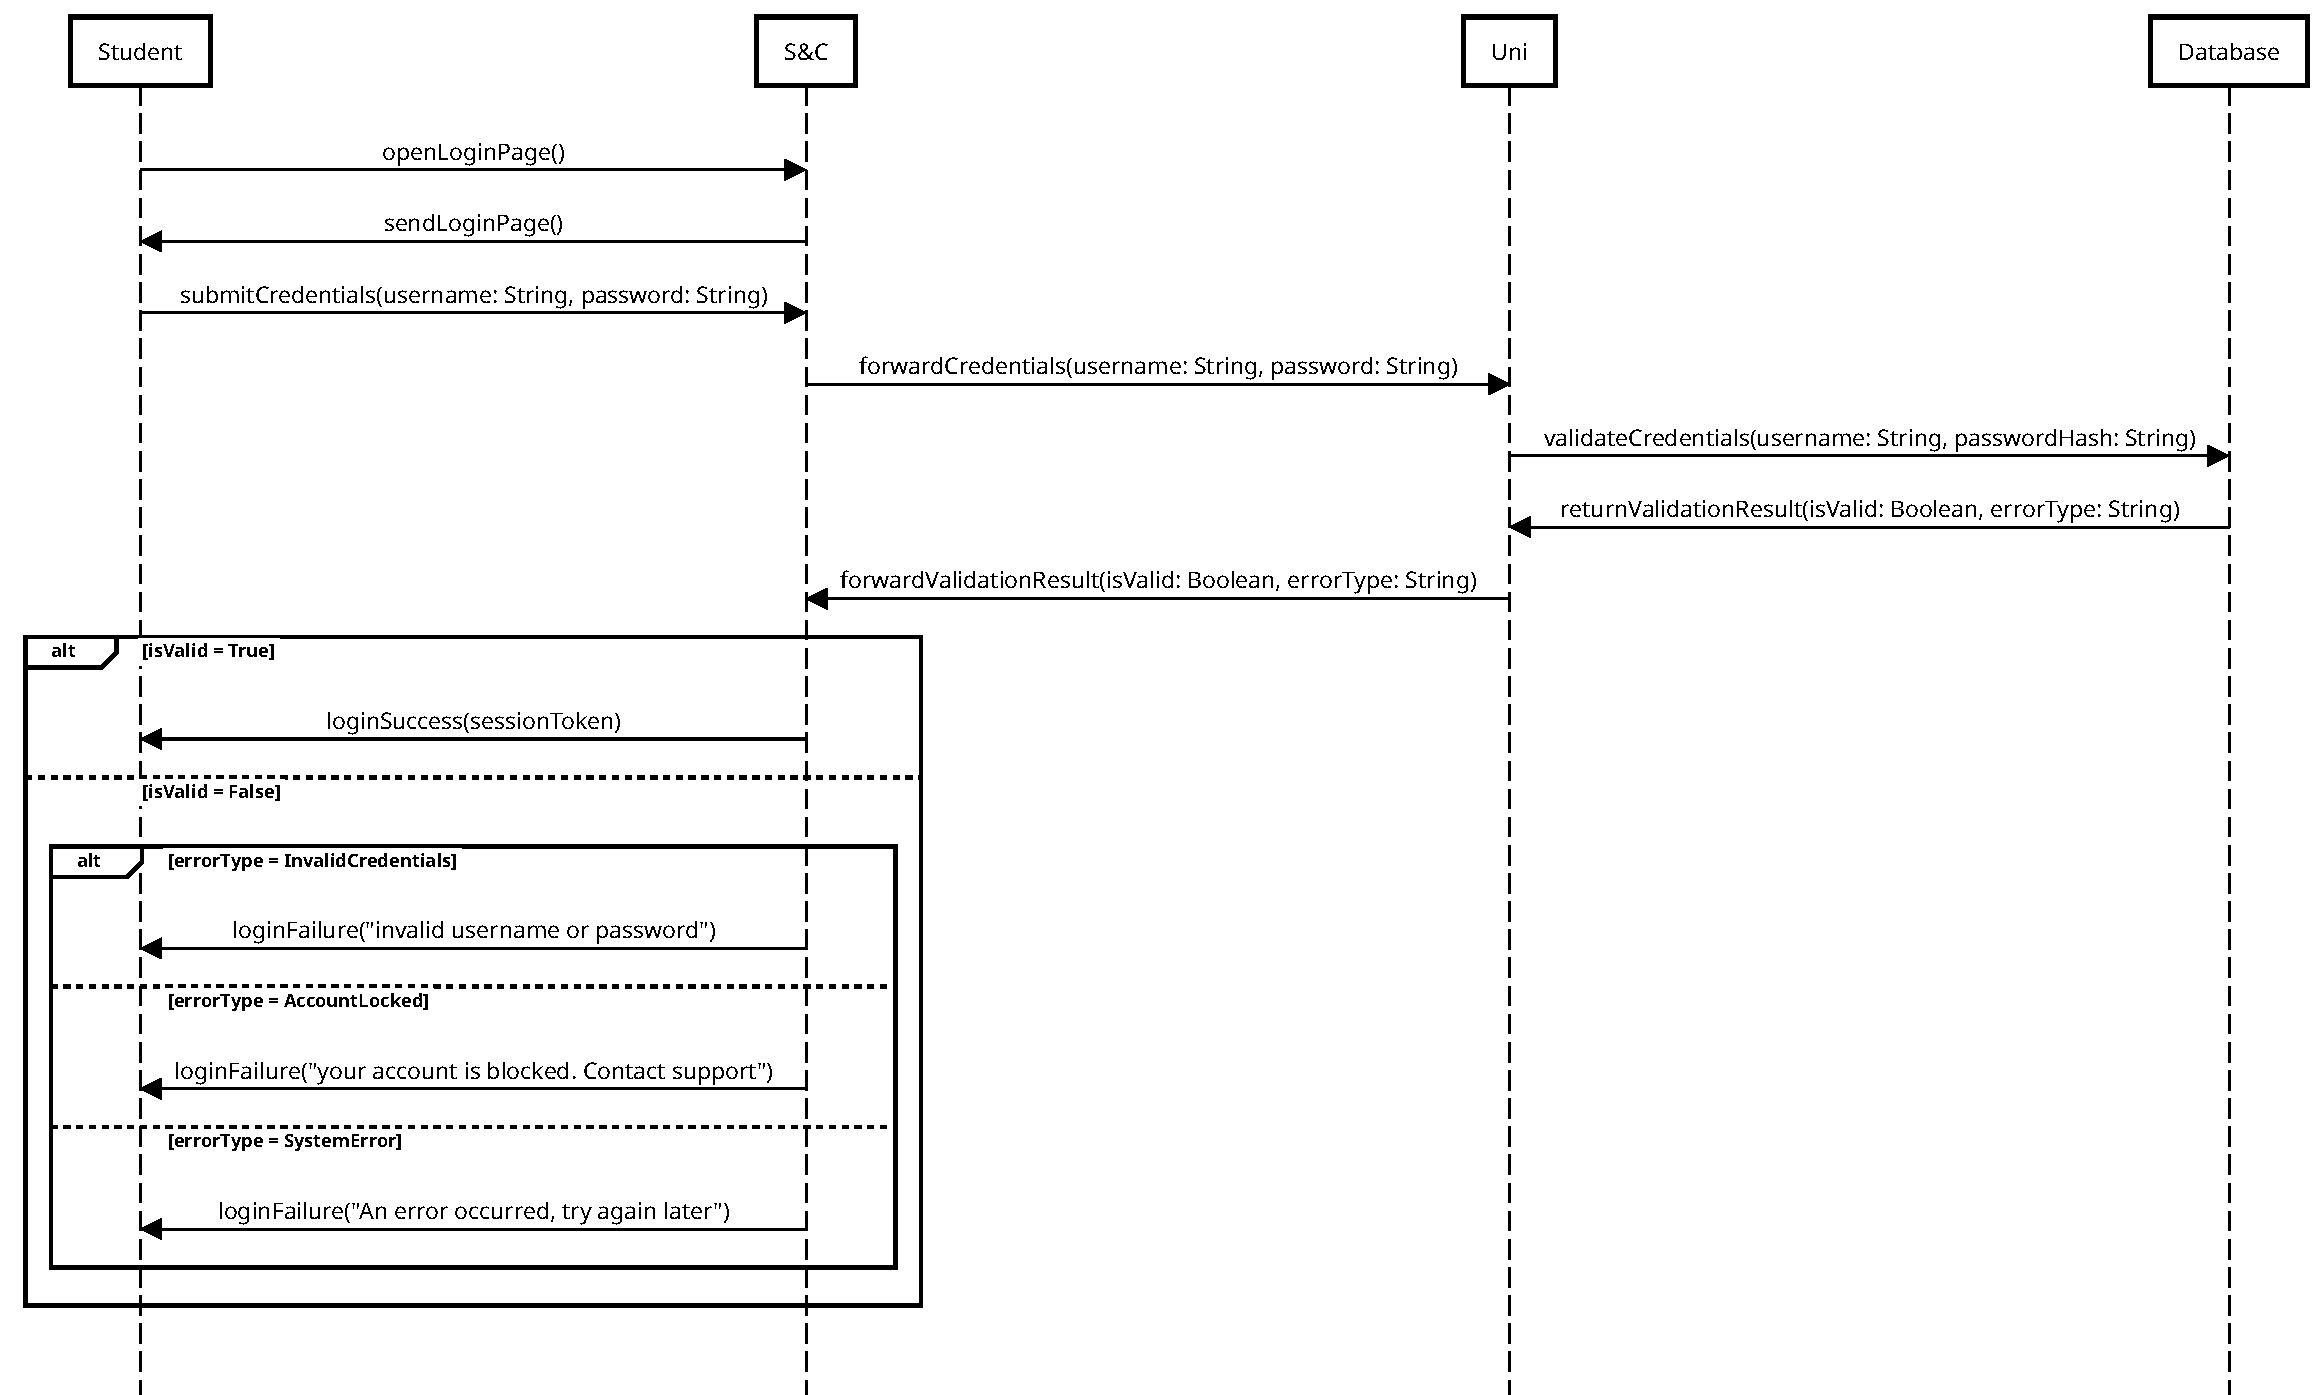
\includegraphics[width=1\textwidth]{Images/UC_1.pdf}
    \caption{Student Login - Use Case Diagram}
    \label{fig:use-case-diagram-1}
\end{figure}

% 2

\subsubsection{UC02: Student uploads its CV and receives suggestions}
\label{subsubsec:studend-upload-CV}
\begin{center}
    \begin{longtable}{|l|p{0.75\linewidth}|}
        \hline
        \textbf{Actors:}           & ST                                                                                                    \\
        \hline
        \textbf{Entry Conditions:} & ST is correctly logged in to S\&C.                                                                    \\
        \hline
        \textbf{Flow of Events:}   & \begin{enumerate}
                                         \item ST visits the "My CV" page.
                                         \item ST uploads the CV file to S\&C.
                                         \item S\&C stores the CV in the database.
                                         \item The insert/update operation on the S\&C database triggers the CV suggestion system.
                                         \item The suggestion system fetches the CV from the database and analyzes it.
                                         \item The suggestion system generates feedback and improvement suggestions and stores them.
                                         \item The ST can see the suggestions by clicking on the "Show suggestions" button on the "My CV" page.
                                     \end{enumerate} \\
        \hline
        \textbf{Exit Conditions:}  & ST has successfully uploaded the CV and received suggestions.                                         \\
        \hline
        \textbf{Exceptions:}       & The ST tries to get the suggestions before they are ready.                                            \\                                                      \\
        \hline
    \end{longtable}
\end{center}

\begin{figure}[H]
    \centering
    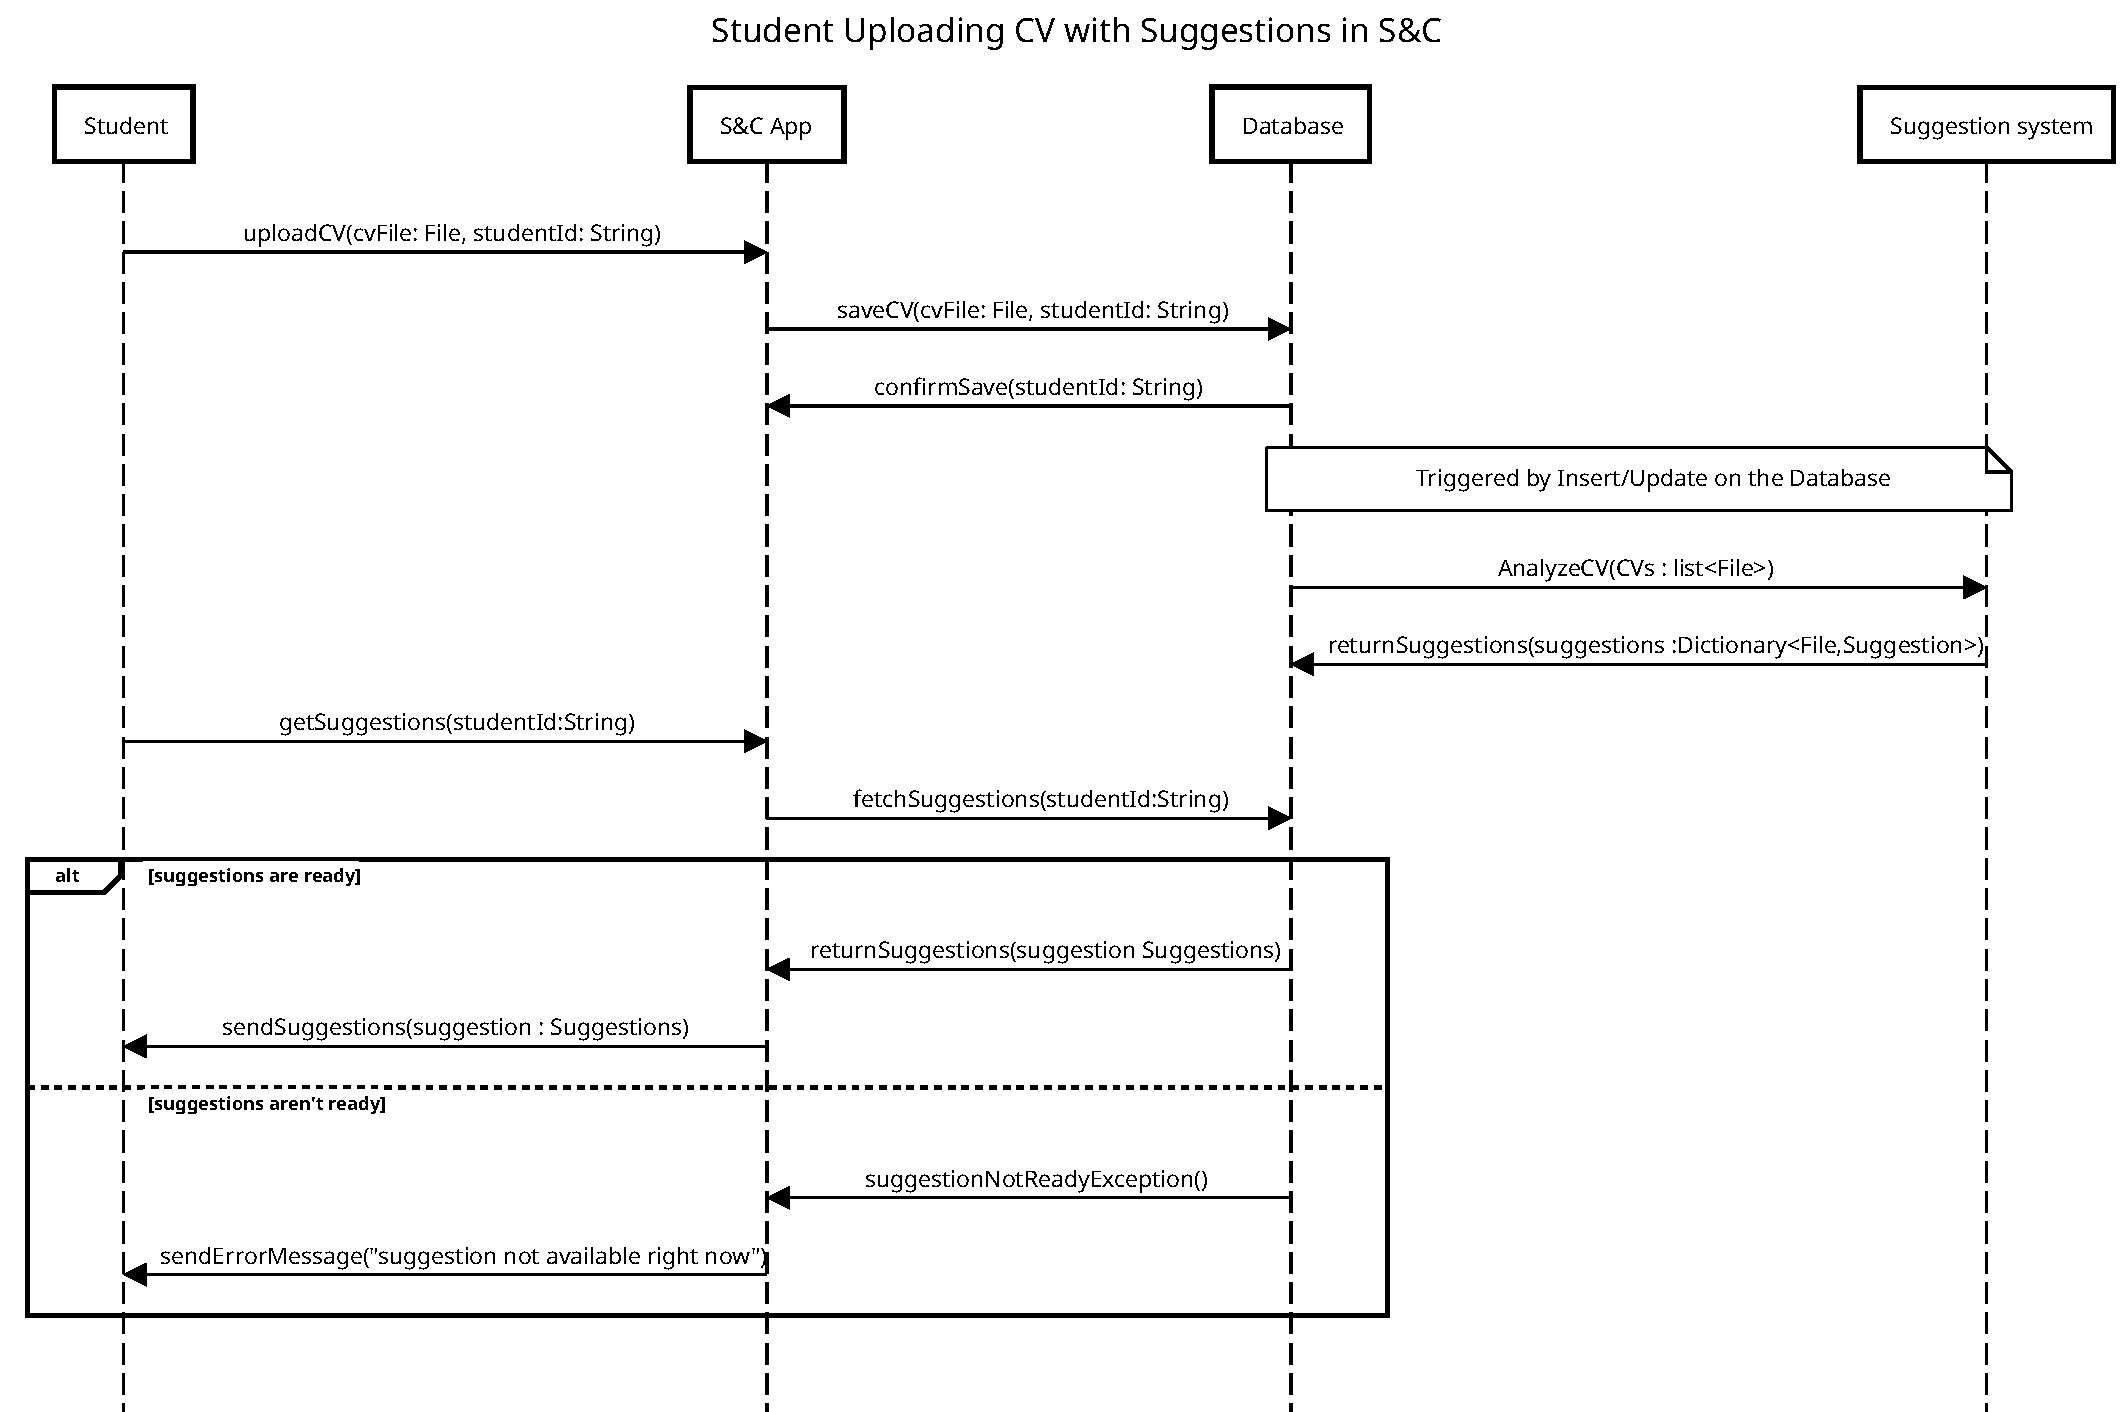
\includegraphics[width=1\textwidth]{Images/UC_2.pdf}
    \caption{Student Uploads its CV and Receives Suggestions - Use Case Diagram}
    \label{fig:use-case-diagram-2}
\end{figure}

% 3

\subsubsection{UC03: Student internship advertisement search}
\label{subsubsec:student-internship-advertisement-search}

\begin{center}
    \begin{longtable}{|l|p{0.75\linewidth}|}
        \hline
        \textbf{Actors:}           & ST                                                        \\
        \hline
        \textbf{Entry Conditions:} & ST is correctly logged in.                                \\
        \hline
        \textbf{Flow of Events:}   & \begin{enumerate}
                                         \item ST visits the "Internships" page.
                                         \item S\&C fetch the internships from the database.
                                         \item S\&C shows the internships to the ST.
                                         \item ST filters the internships by keyword, company, etc.
                                         \item S\&C shows the filtered internships to the ST.
                                         \item ST selects an internship to view the details.
                                         \item S\&C fetch the internship details from the database.
                                         \item S\&C shows the internship details to the ST.
                                     \end{enumerate} \\
        \hline
        \textbf{Exit Conditions:}  & ST has successfully viewed the internships.               \\
        \hline
        \textbf{Exceptions:}       & S\&C generated an internal error.                         \\
        \hline
    \end{longtable}
\end{center}

\begin{figure}[H]
    \centering
    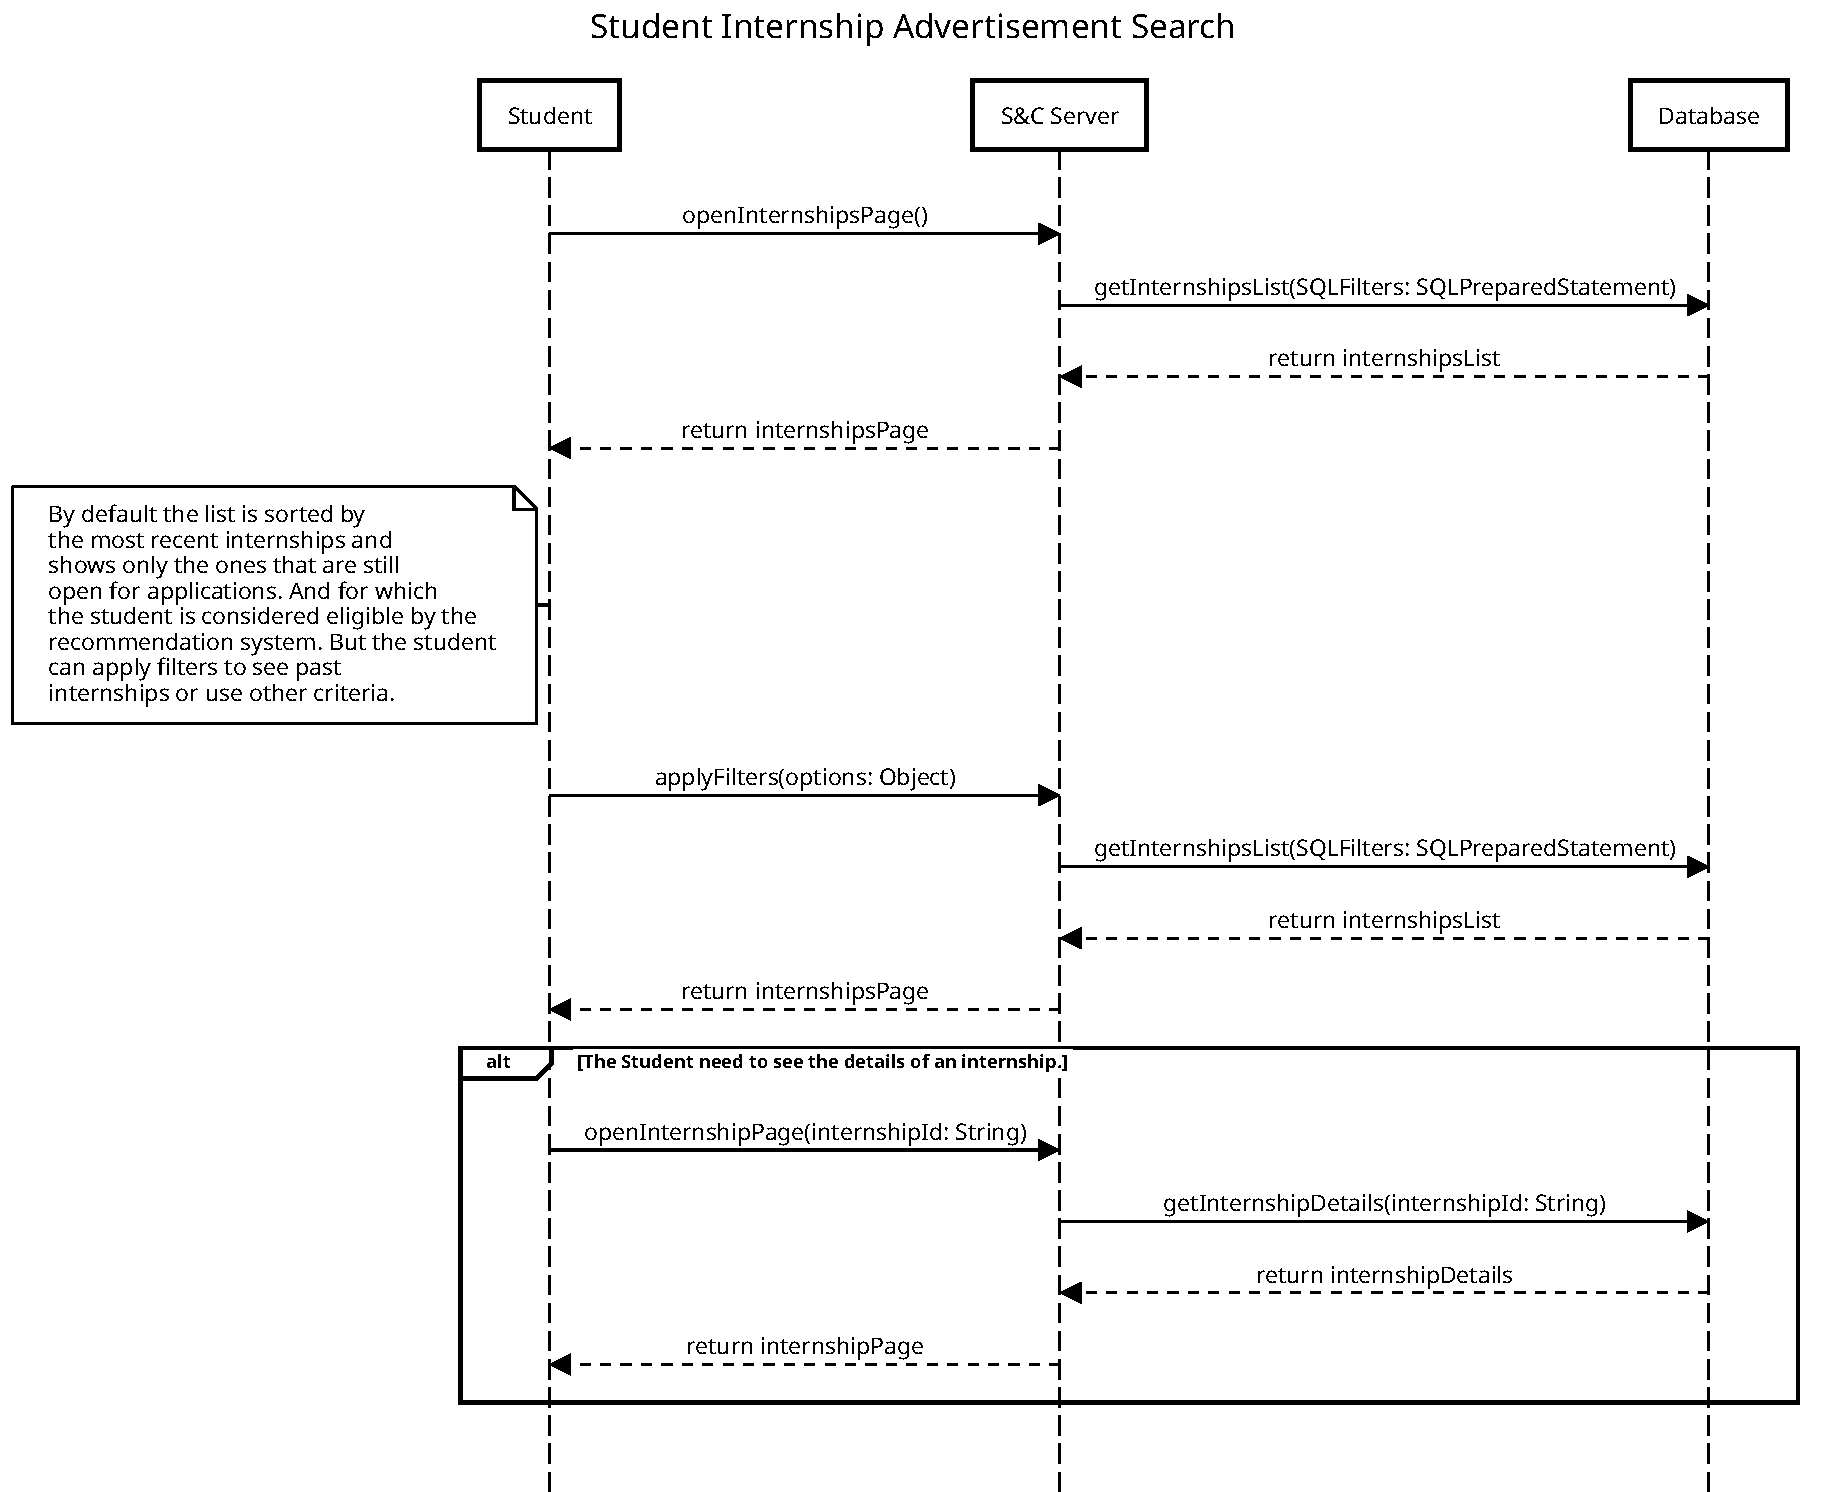
\includegraphics[width=1.0\textwidth]{Images/UC_3.pdf}
    \caption{Student Internship Advertisement Search - Use Case Diagram}
    \label{fig:use-case-diagram-3}
\end{figure}

% 4

\subsubsection{UC04: Student applies to an internship}
\label{subsubsec:student-applies-to-an-internship}

\begin{center}
    \begin{longtable}{|l|p{0.75\linewidth}|}
        \hline
        \textbf{Actors:}           & ST, CO                                                               \\
        \hline
        \textbf{Entry Conditions:} & ST is correctly logged in.                                           \\
        \hline
        \textbf{Flow of Events:}   & \begin{enumerate}
                                         \item ST visits the "Internships" page.
                                         \item S\&C fetch the internships from the database.
                                         \item S\&C shows the internships to the ST.
                                         \item ST selects an internship to view the details.
                                         \item S\&C fetch the internship details from the database.
                                         \item S\&C shows the internship details to the ST.
                                         \item ST clicks on the "Apply" button.
                                         \item S\&C stores the application in the database.
                                         \item S\&C notifies the CO that the ST has applied to the internship.
                                     \end{enumerate} \\
        \hline
        \textbf{Exit Conditions:}  & ST has successfully applied to the internship.                       \\
        \hline
        \textbf{Exceptions:}       & S\&C generated an internal error.                                    \\
        \hline
    \end{longtable}
\end{center}

\begin{figure}[H]
    \centering
    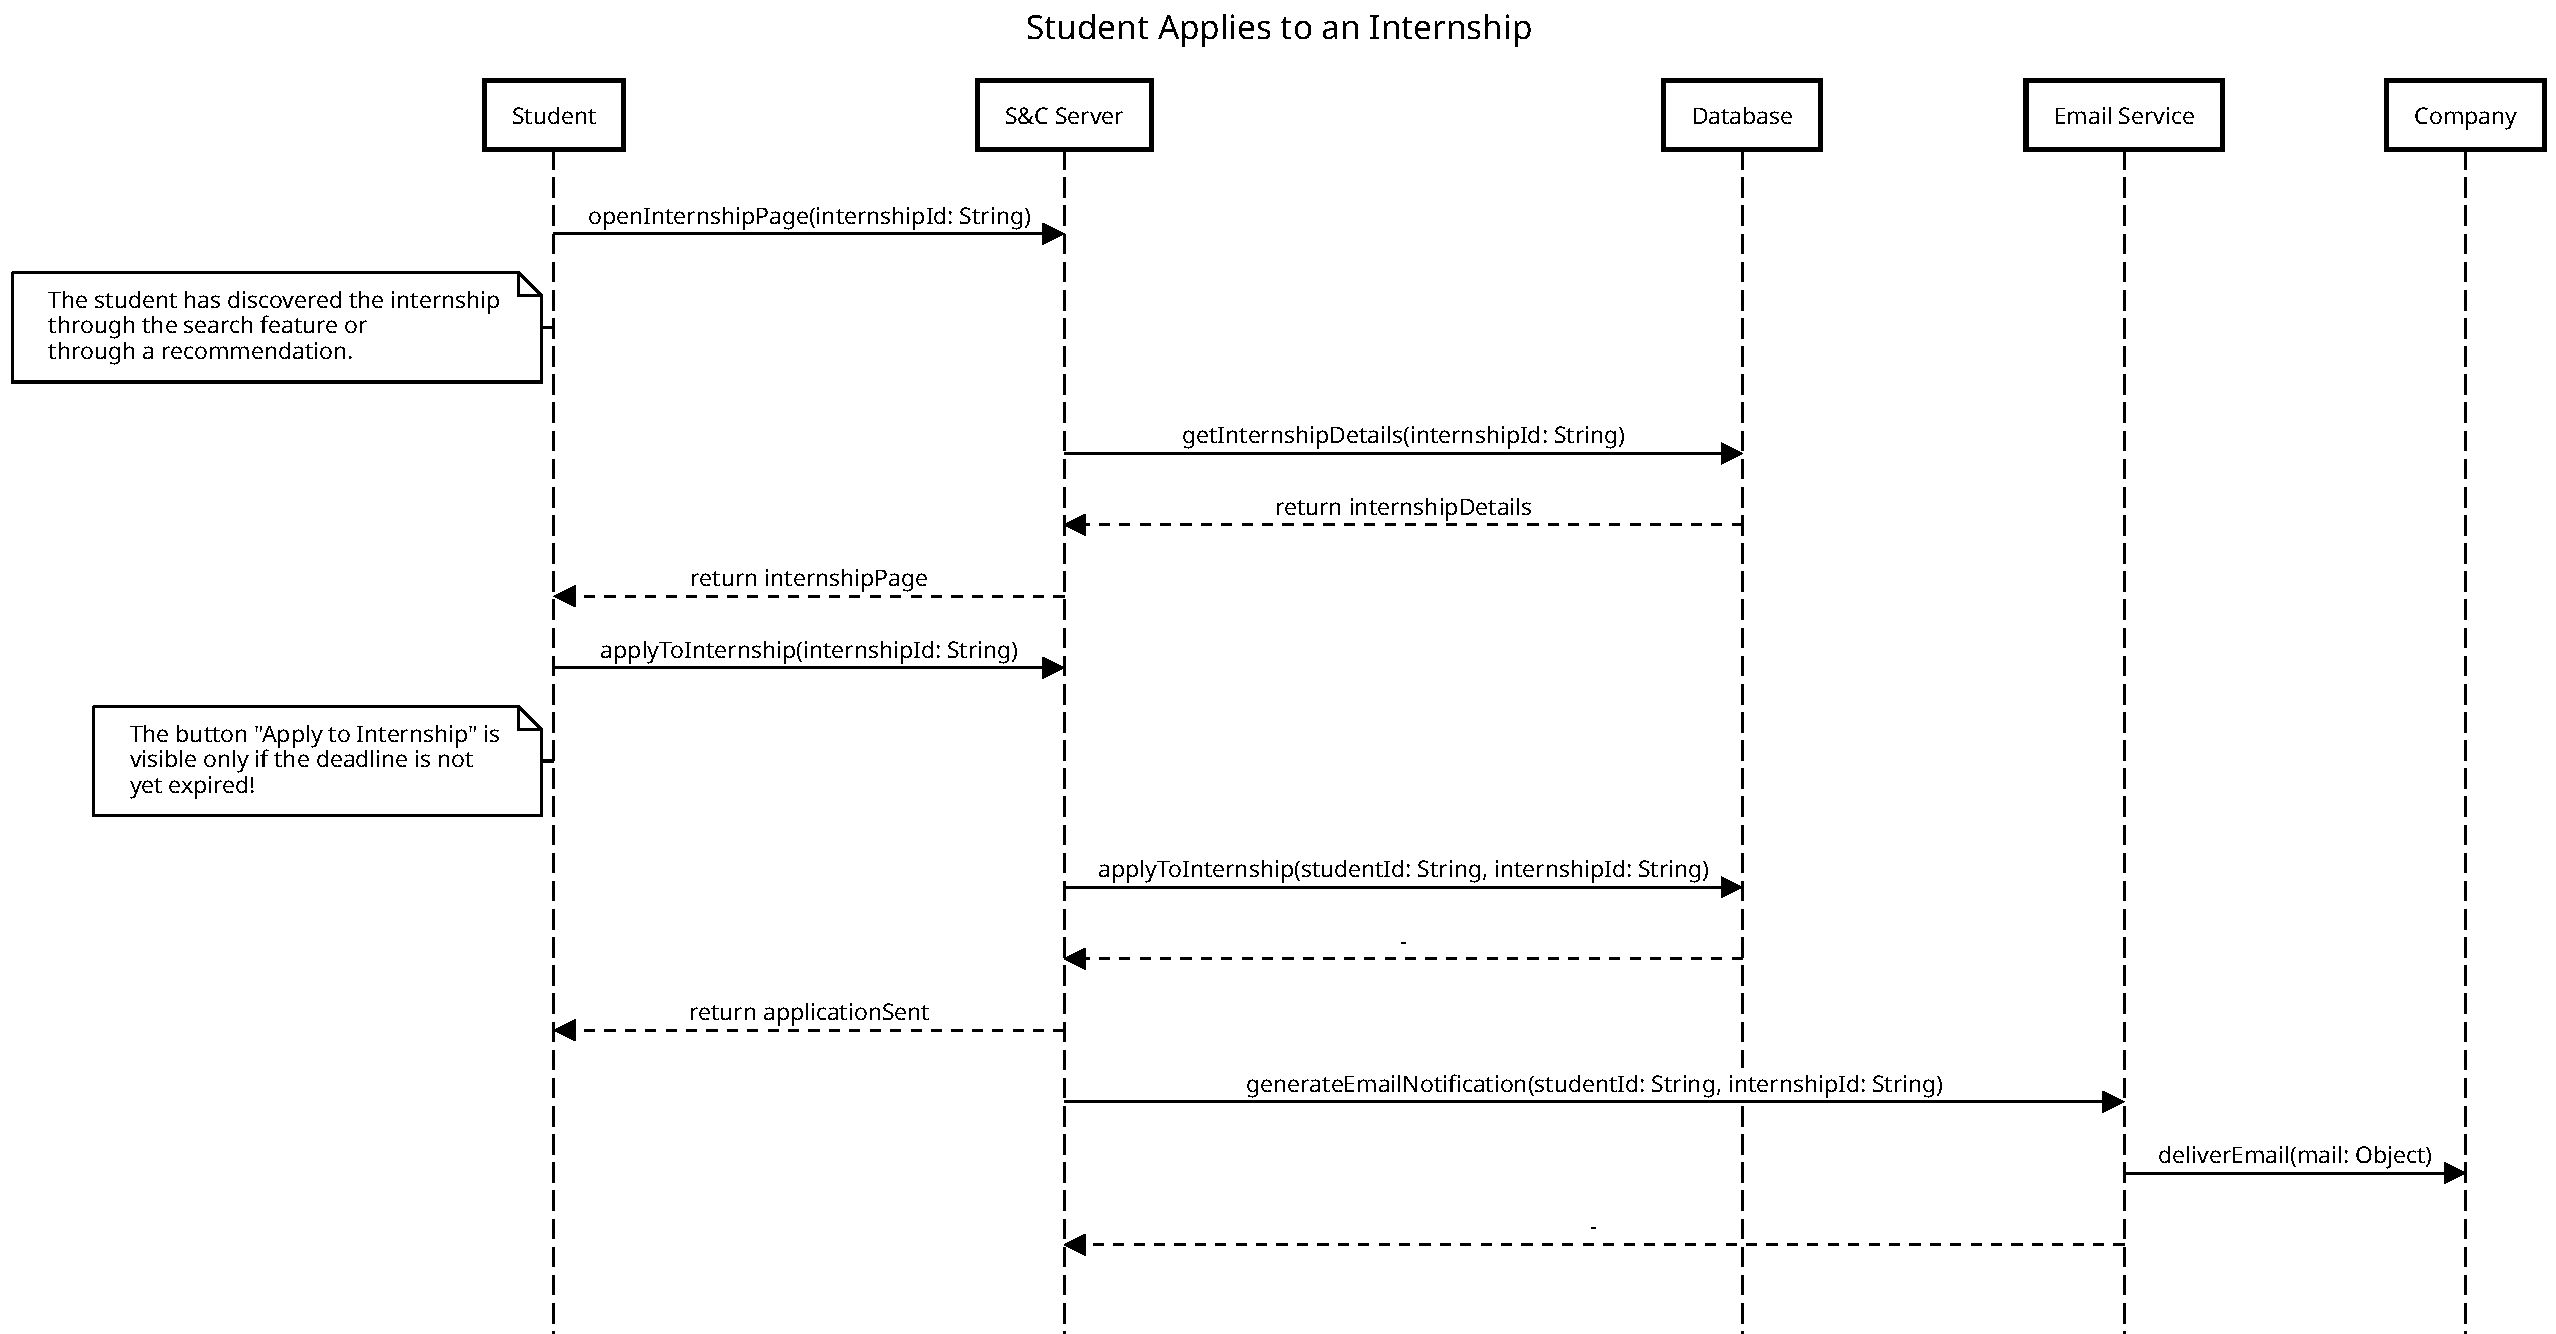
\includegraphics[width=1.0\textwidth]{Images/UC_4.pdf}
    \caption{Student Applies to an Internship - Use Case Diagram}
    \label{fig:use-case-diagram-4}
\end{figure}

% 5

\subsubsection{UC05: Student answers a company questionnaire}
\label{subsubsec:student-answers-a-company-questionnaire}

\begin{center}
    \begin{longtable}{|l|p{0.75\linewidth}|}
        \hline
        \textbf{Actors:}           & ST, CO                                                                             \\
        \hline
        \textbf{Entry Conditions:} & CO has requested ST to fill a questionnaire.                                       \\
        \hline
        \textbf{Flow of Events:}   & \begin{itemize}
                                         \item (opt. 1) ST uses the link sent by S\&C via email to access the questionnaire.
                                               \begin{enumerate}
                      \item S\&C verify if the link is valid.
                            \begin{itemize}
                                \item Link valid and not expired: the flow continues.
                                \item Link invalid or expired: ST is redirected to the questionnaire page.
                            \end{itemize}
                  \end{enumerate}
                                         \item (opt. 2) ST finds the questionnaire directly on the S\&C platform.
                                               \begin{enumerate}
                      \item ST visits the "My Internships" page.
                      \item S\&C fetch the internships from the database.
                      \item S\&C shows the internships to the ST.
                      \item ST selects an internship to view the details.
                      \item S\&C fetch the internship details from the database.
                      \item S\&C shows the internship details to the ST.
                      \item ST clicks on the "Compile the Questionnaire" button.
                      \item ST is redirected to the questionnaire page.
                  \end{enumerate}
                                         \item S\&C fetch the questionnaire from the database.
                                         \item S\&C shows the questionnaire to the ST.
                                         \item ST starts to fill the questionnaire. For each question:
                                               \begin{enumerate}
                      \item ST gives an answer.
                      \item S\&C stores the answer in the database.
                  \end{enumerate}
                                         \item ST ends its job and submits the questionnaire.
                                         \item S\&C stores that the questionnaire was submitted.
                                         \item S\&C notifies the CO that the questionnaire was successfully submitted.
                                         \item S\&C sends a notification email to the CO about the questionnaire submission.
                                         \item S\&C evaluates the answers and compute the final score.
                                         \item S\&C the final score is stored to be consulted by the CO later.
                                     \end{itemize} \\
        \hline
        \textbf{Exit Conditions:}  & ST has successfully filled the questionnaire.                                      \\
        \hline
        \textbf{Exceptions:}       & S\&C generated an internal error. The link is invalid or expired.                  \\
        \hline
    \end{longtable}
\end{center}

\begin{figure}[H]
    \centering
    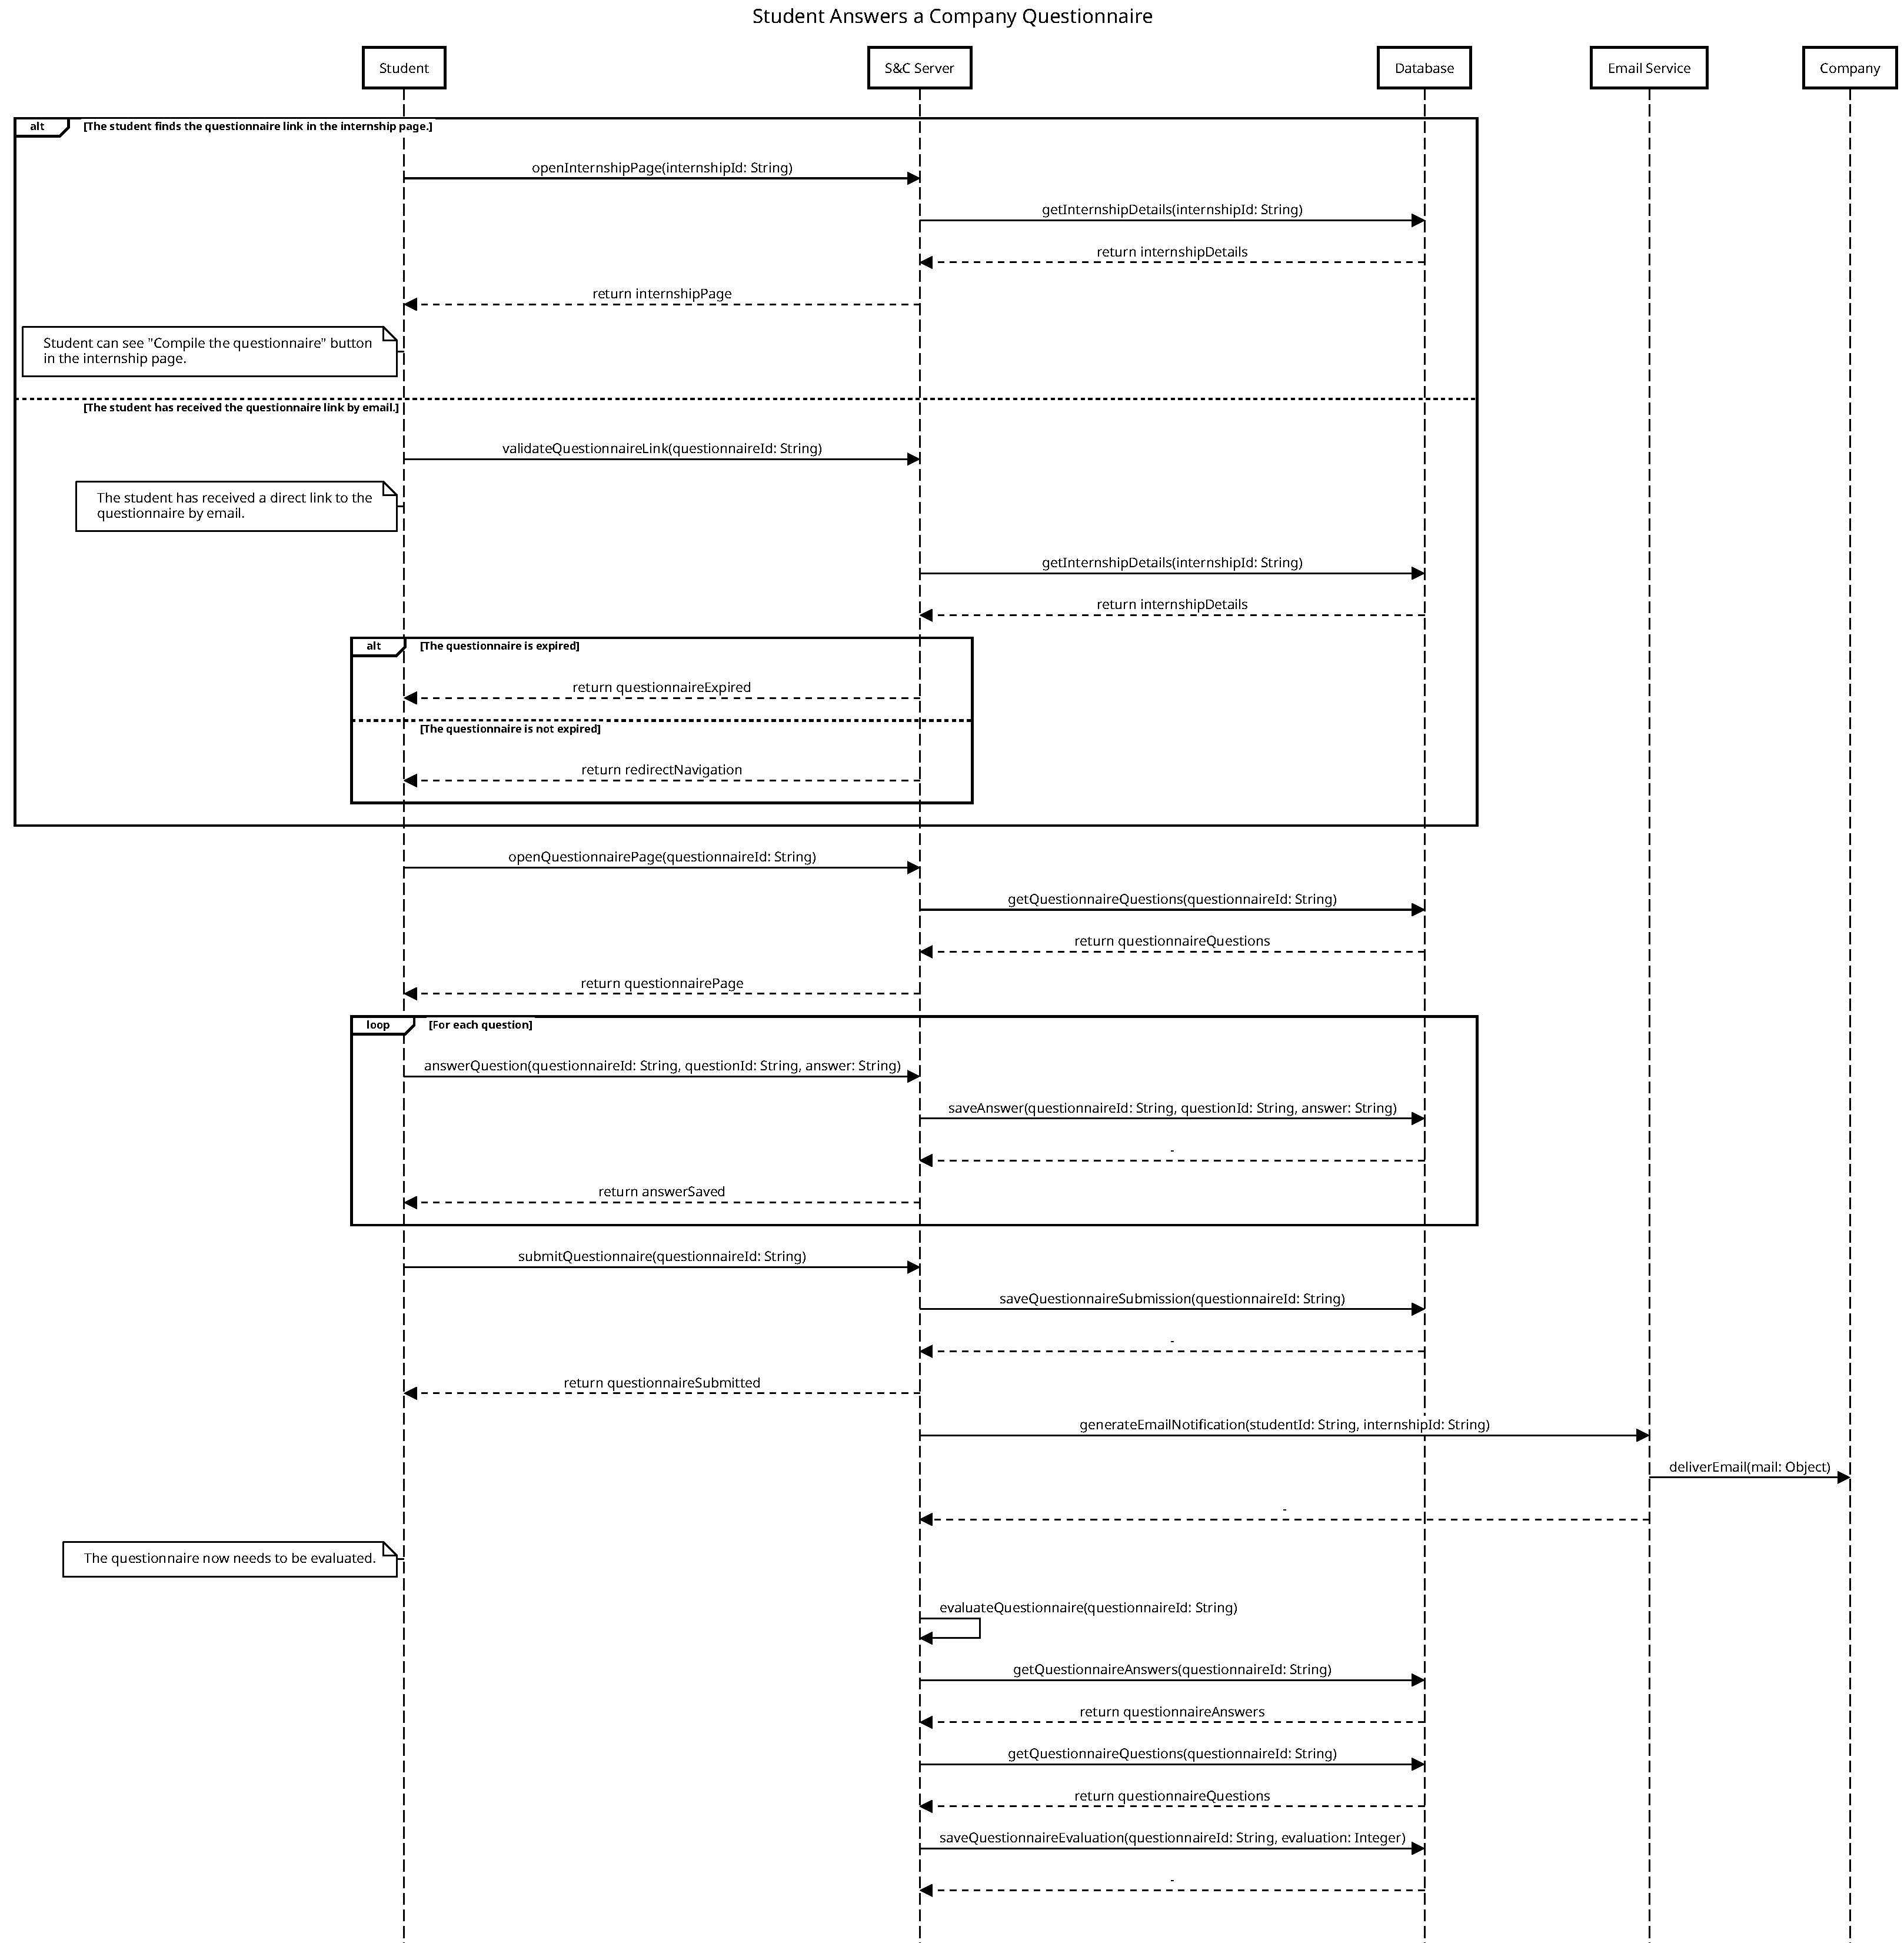
\includegraphics[width=1.0\textwidth]{Images/UC_5.pdf}
    \caption{Student Answers a Company Questionnaire - Use Case Diagram}
    \label{fig:use-case-diagram-5}
\end{figure}

% 6	

\subsubsection{UC06: Student creates a complaints}
\label{subsubsec:student-creates-a-complaints}

\begin{center}
    \begin{longtable}{|l|p{0.75\linewidth}|}
        \hline
        \textbf{Actors:}           & ST, (opt) UN                                                                                                                     \\
        \hline
        \textbf{Entry Conditions:} & The ST is correctly logged in. The ST had decided to create a complaint about the internship he's doing.                         \\
        \hline
        \textbf{Flow of Events:}   & \begin{enumerate}
                                         \item ST clicks on the "Create Complaint" button.
                                         \item S\&C send to the ST a form to fill with the complaint details.
                                         \item ST fills the form and submits it.
                                         \item S\&C stores the complaint in the database.
                                         \item S\&C request to the Emailing system to send an email to the UN about a new complaint about an internship of one of it's ST.
                                         \item The Emailing system sends the email to the UN.
                                         \item S\&C notifies the ST that the complaint was successfully submitted.
                                         \item (opt) UN acknowledges the complaint.
                                         \item (opt) S\&C change the status of the complaint to "Acknowledged".
                                     \end{enumerate} \\
        \hline
        \textbf{Exit Conditions:}  & ST receive the confirmation of the complaint being saved correctly.                                                              \\
        \hline
        \textbf{Exceptions:}       & S\&C generated an internal error.                                                                                                \\
        \hline
    \end{longtable}
\end{center}

\begin{figure}[H]
    \centering
    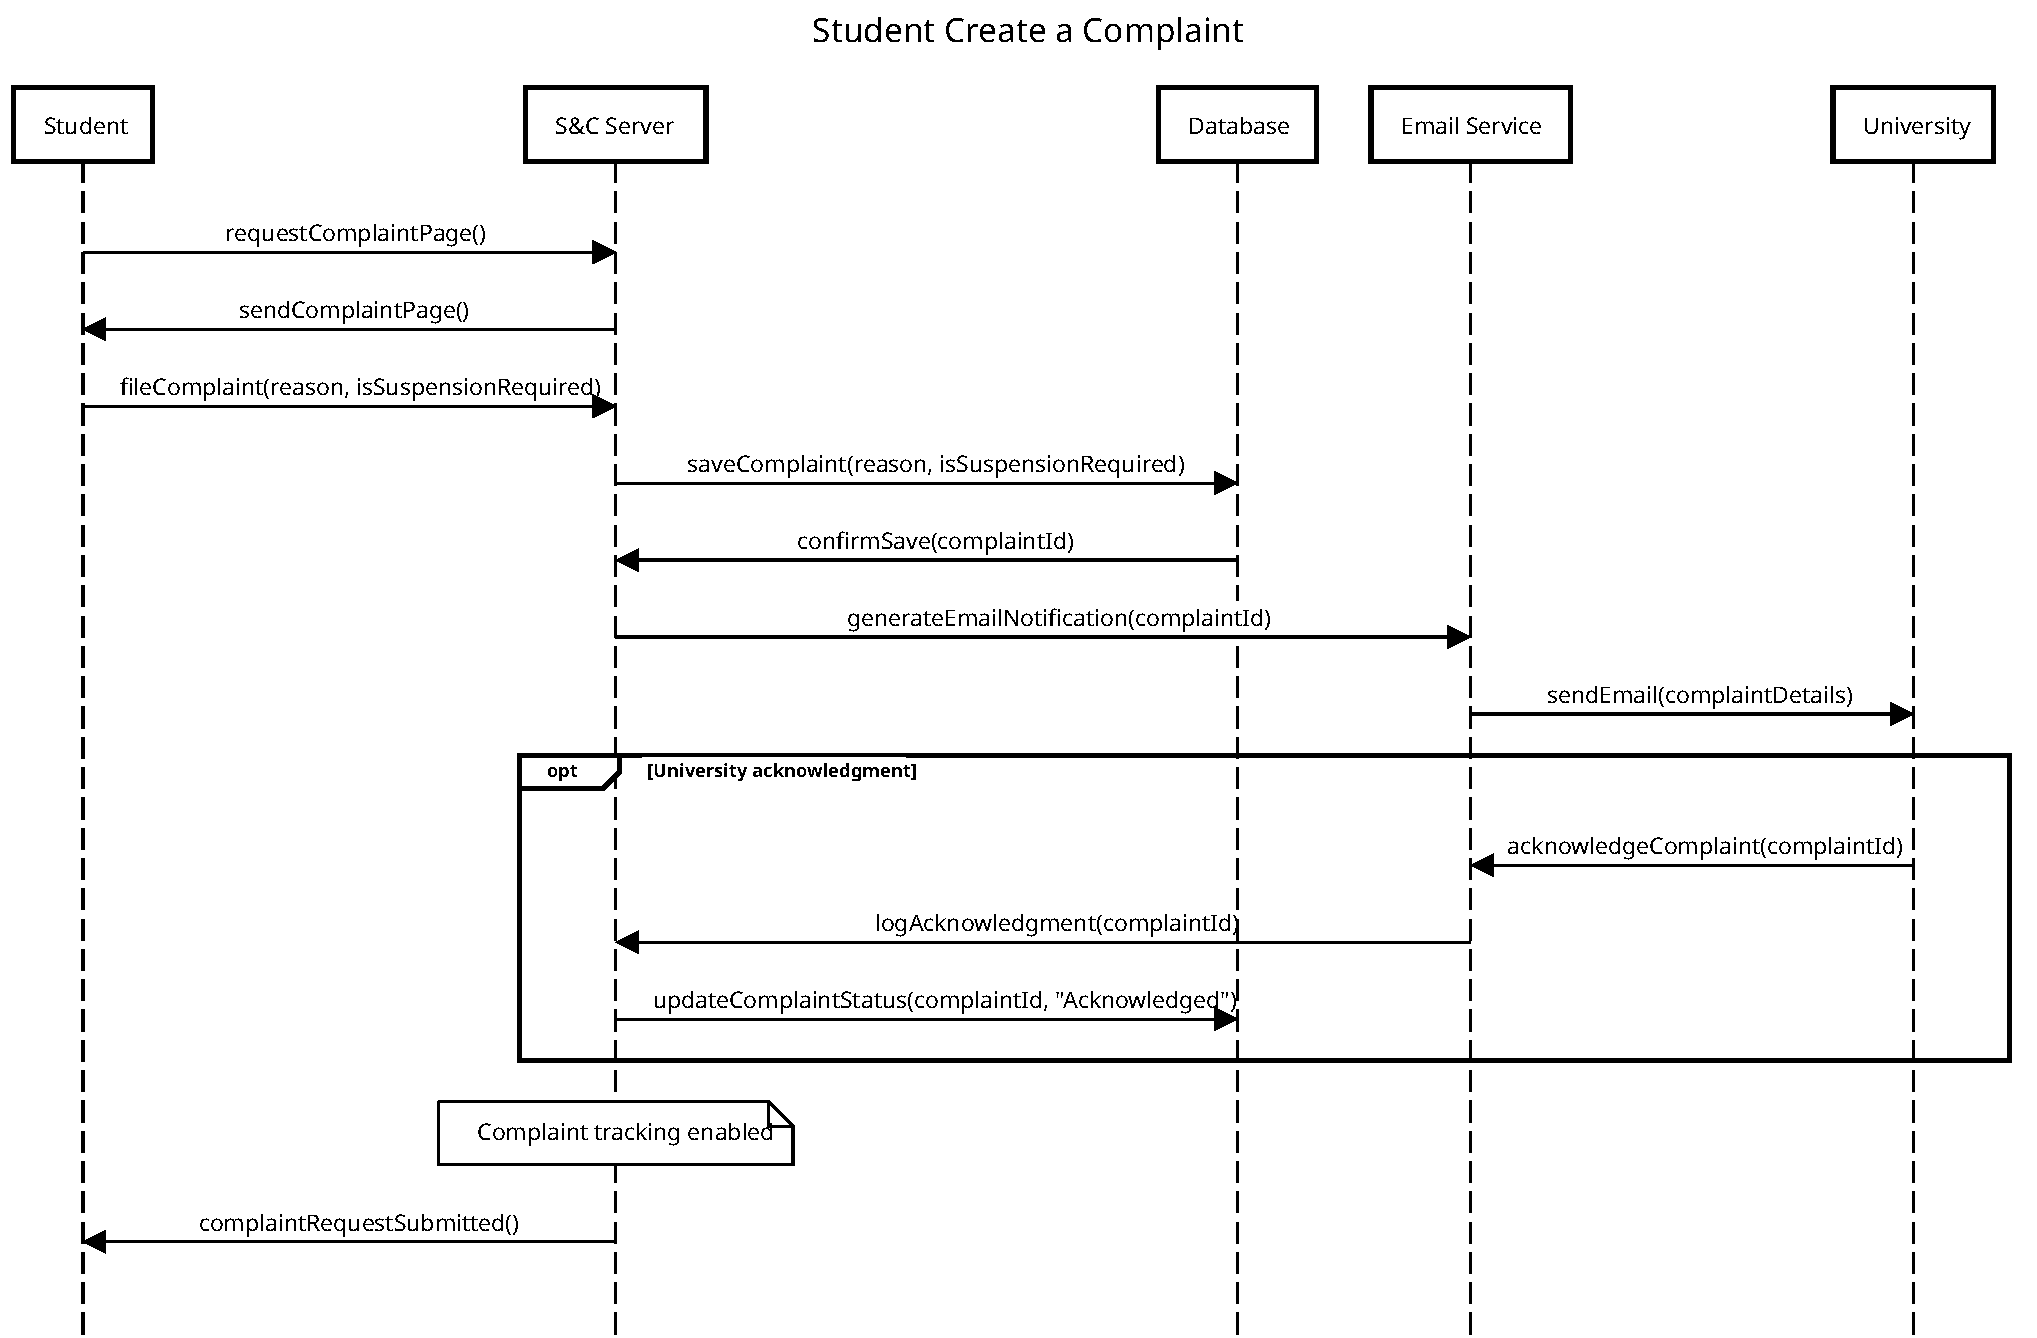
\includegraphics[width=1.0\textwidth]{Images/UC_6.pdf}
    \caption{Student Creates a Complaint - Use Case Diagram}
    \label{fig:use-case-diagram-6}
\end{figure}

% 7

\subsubsection{UC07: Student answers questionnaire at internship completion}
\label{subsubsec:student-answers-questionnaire-at-internship-completion}

\begin{center}
    \begin{longtable}{|l|p{0.75\linewidth}|}
        \hline
        \textbf{Actors:}           & ST                                                                                                     \\
        \hline
        \textbf{Entry Conditions:} & ST is correctly logged in. The related internship has ended.                                           \\
        \hline
        \textbf{Flow of Events:}   & \begin{enumerate}
                                         \item ST clicks on the "Fill Questionnaire" button.
                                         \item S\&C fetch the questionnaire from its database.
                                         \item S\&C gives the questionnaire to the ST.
                                         \item ST fills the questions and submits them.
                                         \item S\&C stores the answers to the questionnaire in the database.
                                         \item S\&C feeds the answers of the questionnaire to the suggestion system to learn from this new data.
                                     \end{enumerate} \\
        \hline
        \textbf{Exit Conditions:}  & ST receive the confirmation of the questionnaire being saved correctly.                                \\
        \hline
        \textbf{Exceptions:}       & Possible invalid formats for the answers submitted by the ST.                                          \\
        \hline
    \end{longtable}
\end{center}

\begin{figure}[H]
    \centering
    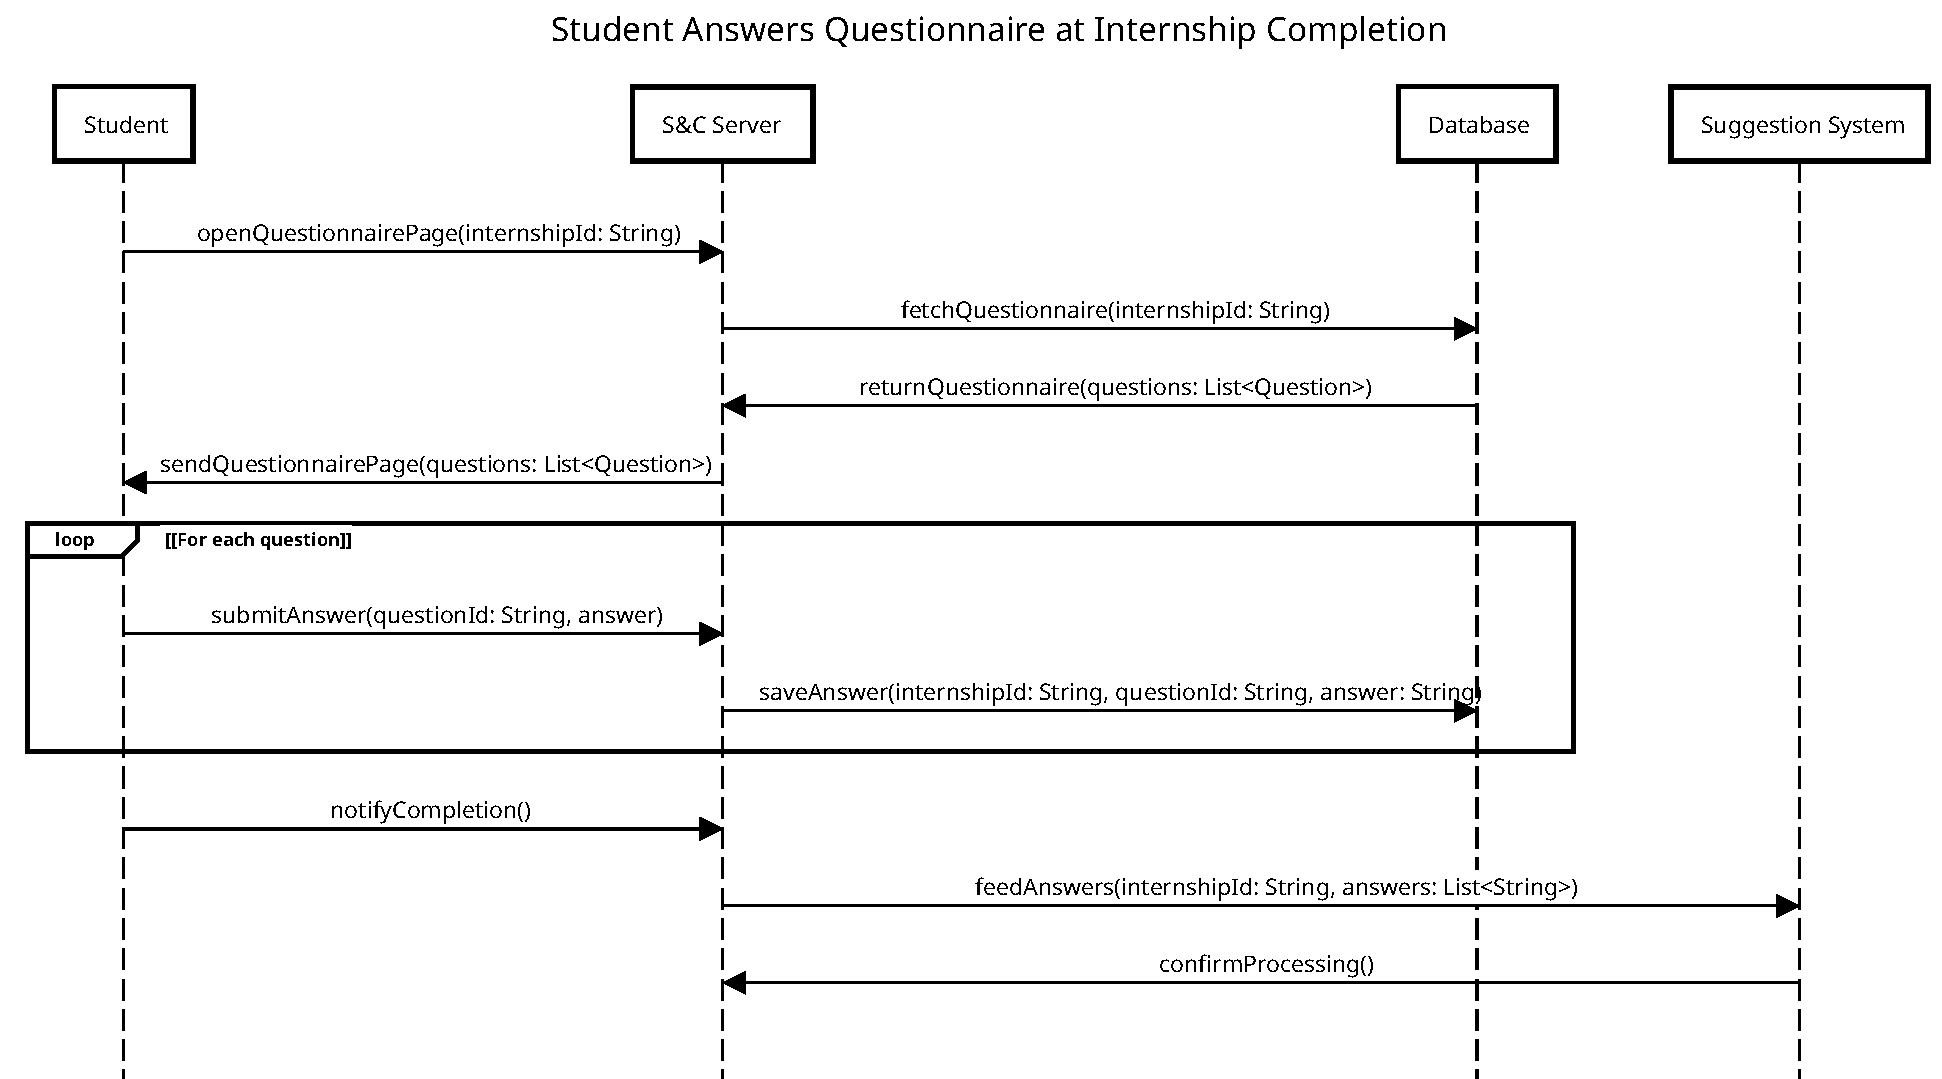
\includegraphics[width=1.0\textwidth]{Images/UC_7.pdf}
    \caption{Student Answers Questionnaire at Internship Completion - Use Case Diagram}
    \label{fig:use-case-diagram-7}
\end{figure}

% 8

\subsubsection{UC08: Company login}
\label{subsubsec:company-login}

\begin{center}
    \begin{longtable}{|l|p{0.75\linewidth}|}
        \hline
        \textbf{Actors:}           & CO                                                                                            \\
        \hline
        \textbf{Entry Conditions:} & CO has received the credentials by S\&C staff after the payment for the usage of the Website. \\
        \hline
        \textbf{Flow of Events:}   & \begin{enumerate}
                                         \item CO search the URL of S\&C login page.
                                         \item S\&C send to CO the login web page.
                                         \item CO inserts the username and password received.
                                         \item S\&C validates the credentials.
                                         \item S\&C sends the CO to the CO dashboard.
                                     \end{enumerate}                                           \\
        \hline
        \textbf{Exit Conditions:}  & CO is redirected to the CO dashboard.                                                         \\
        \hline
        \textbf{Exceptions:}       &
        \begin{itemize}
            \item The credentials are wrong.
            \item The CO is was blocked by the S\&C staff after a violation of the platform guidelines.
            \item S\&C generated an internal error.
        \end{itemize}                                 \\
        \hline
    \end{longtable}
\end{center}

\begin{figure}[H]
    \centering
    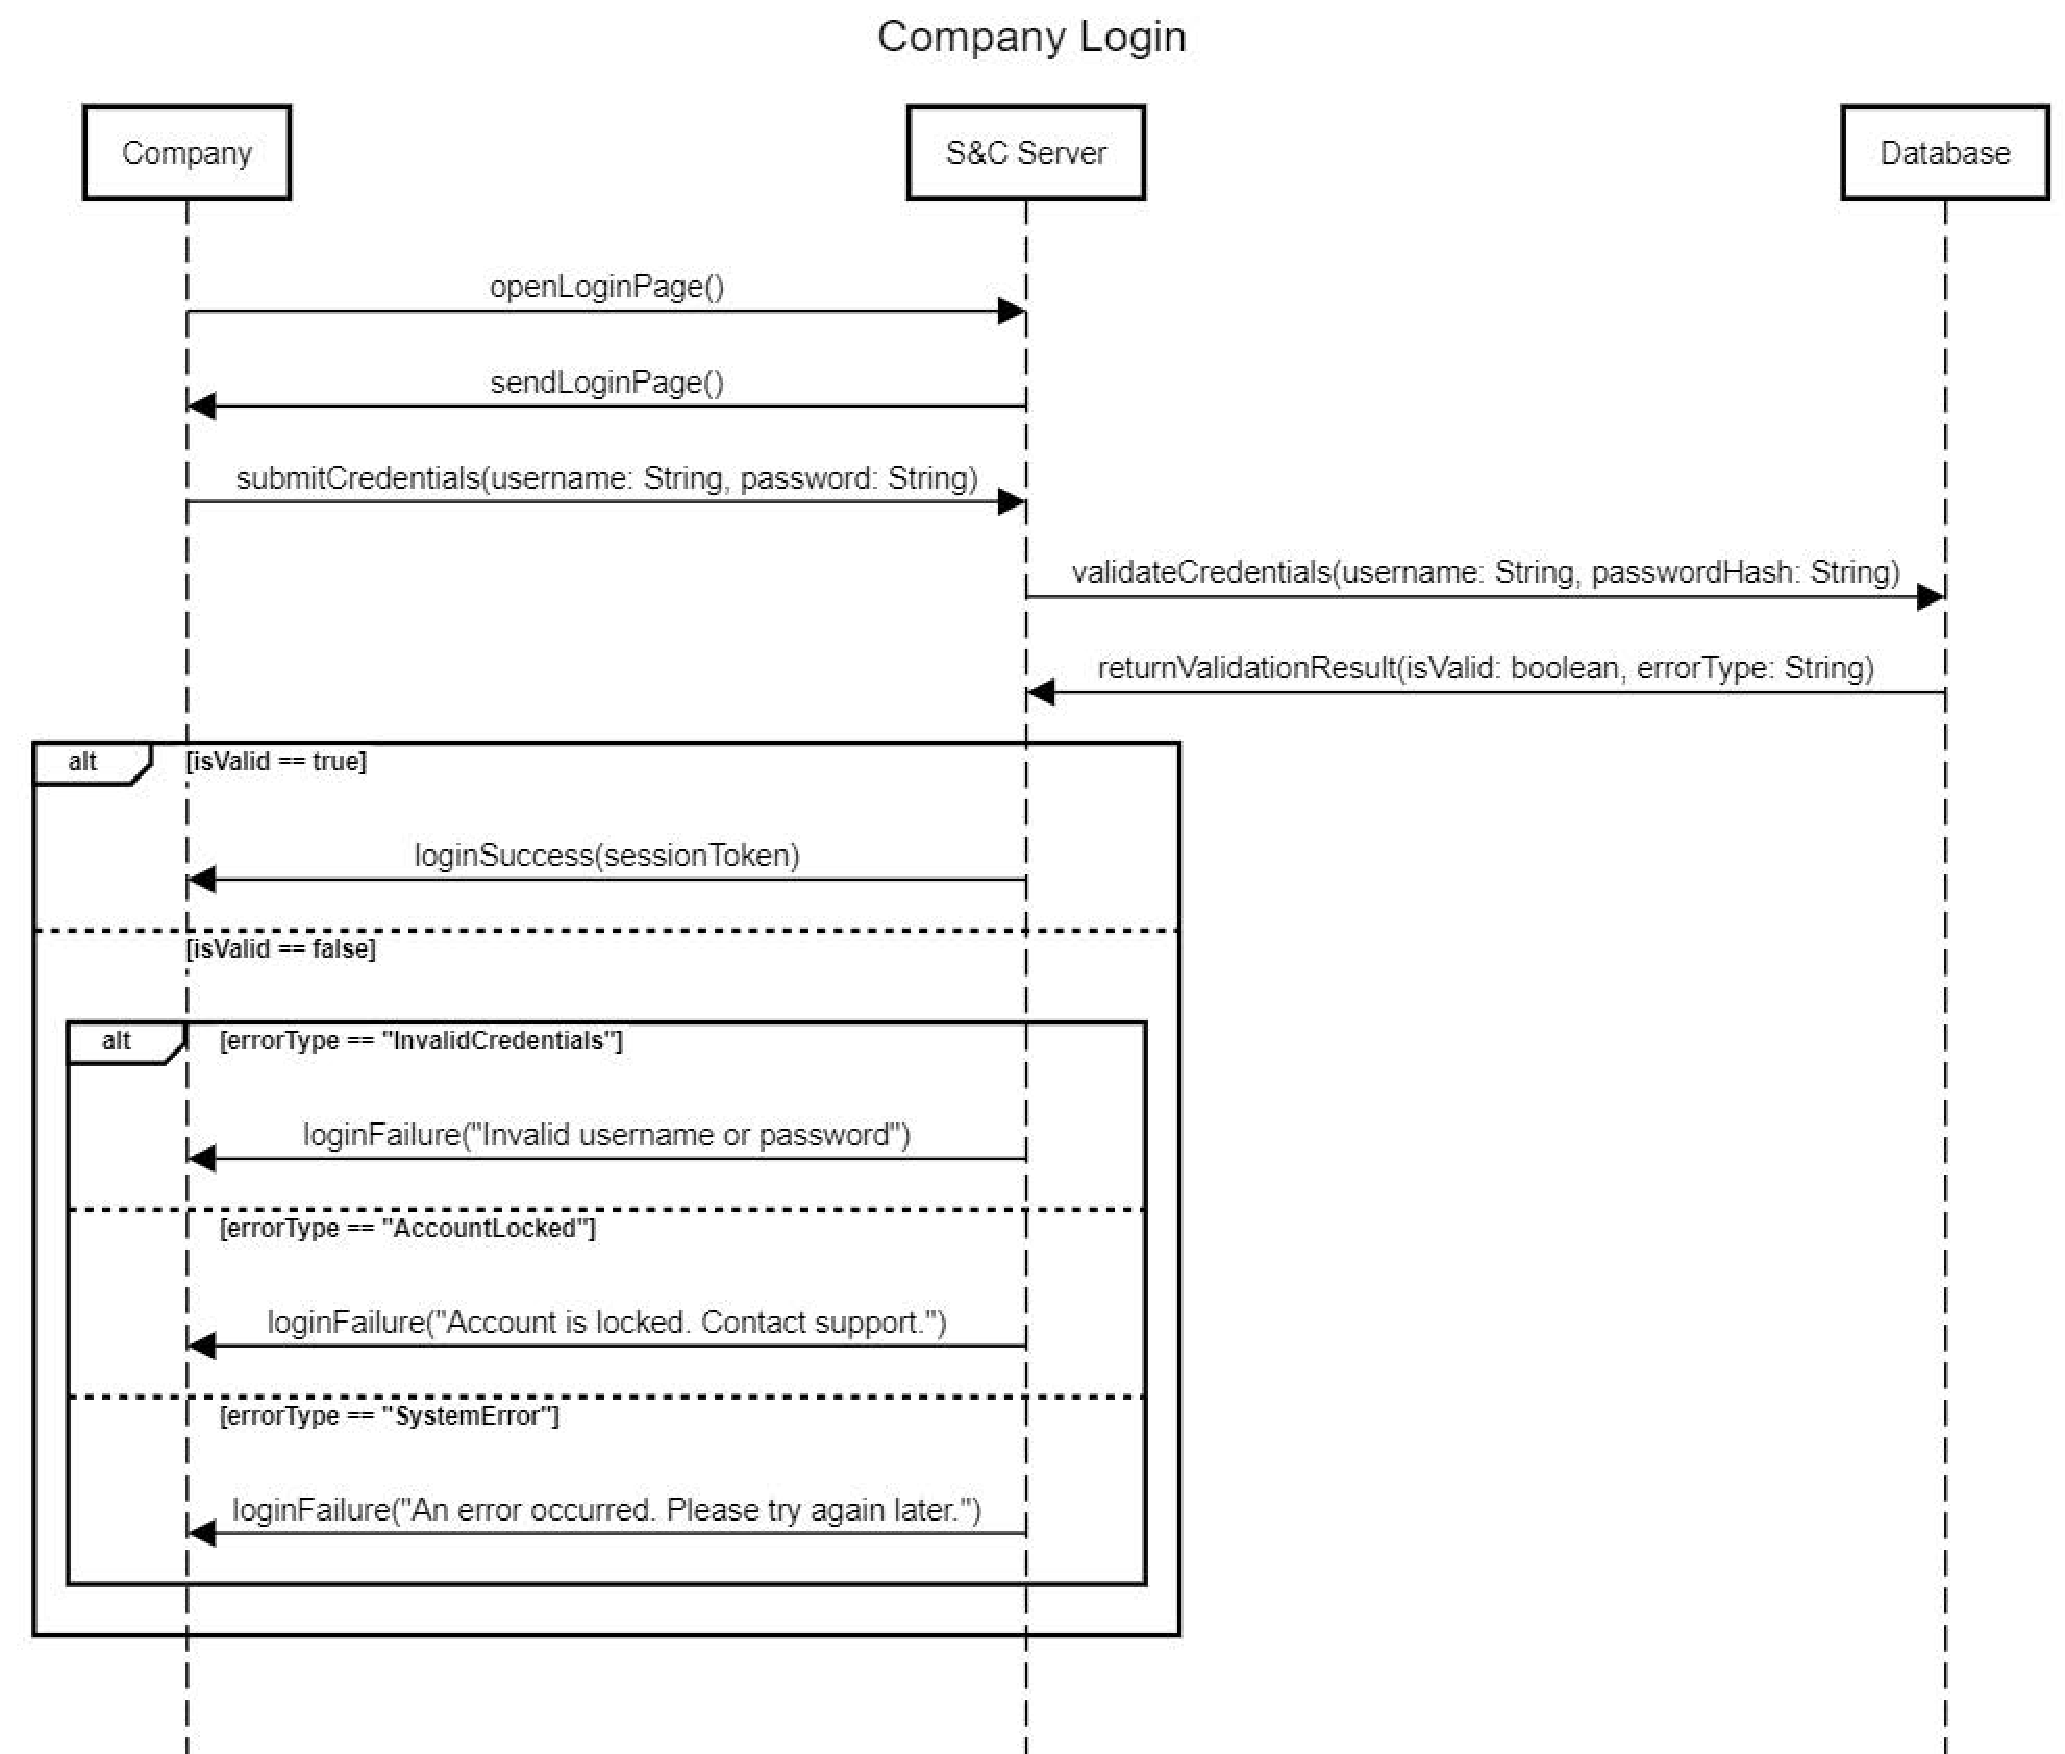
\includegraphics[width=1\textwidth]{Images/UC_8.pdf}
    \caption{Company Login - Use Case Diagram}
    \label{fig:use-case-diagram-8}
\end{figure}

% 9

\subsubsection{UC09: Company creates an internship announcement}
\label{subsubsec:company-creates-an-internship-announcement}

\begin{center}
    \begin{longtable}{|l|p{0.75\linewidth}|}
        \hline
        \textbf{Actors:}           & CO                                                                                                                                                 \\                                                                                       \\
        \hline
        \textbf{Entry Conditions:} & CO is correctly logged in.                                                                                                                         \\
        \hline
        \textbf{Flow of Events:}   & \begin{enumerate}
                                         \item CO opens the page "Create Internship".
                                         \item CO compiles all the required fields for the internship.
                                         \item S\&C saves the internship in the database, it is now visible to students.
                                         \item CO can at any time decide to open the internship and start receiving applications. CO is required to provide a Deadline for the applications.
                                         \item S\&C suggestion system provides to CO a set of candidates that could be suitable for the internship.
                                         \item When the deadline is reached, the internship is automatically closed.
                                     \end{enumerate} \\
        \hline
        \textbf{Exit Conditions:}  & CO has successfully created an internship announcement or a partial version was saved.                                                             \\
        \hline
        \textbf{Exceptions:}       & S\&C generated an internal error.                                                                                                                  \\
        \hline                                                                                                                                                                          \\
    \end{longtable}
\end{center}

\begin{figure}[H]
    \centering
    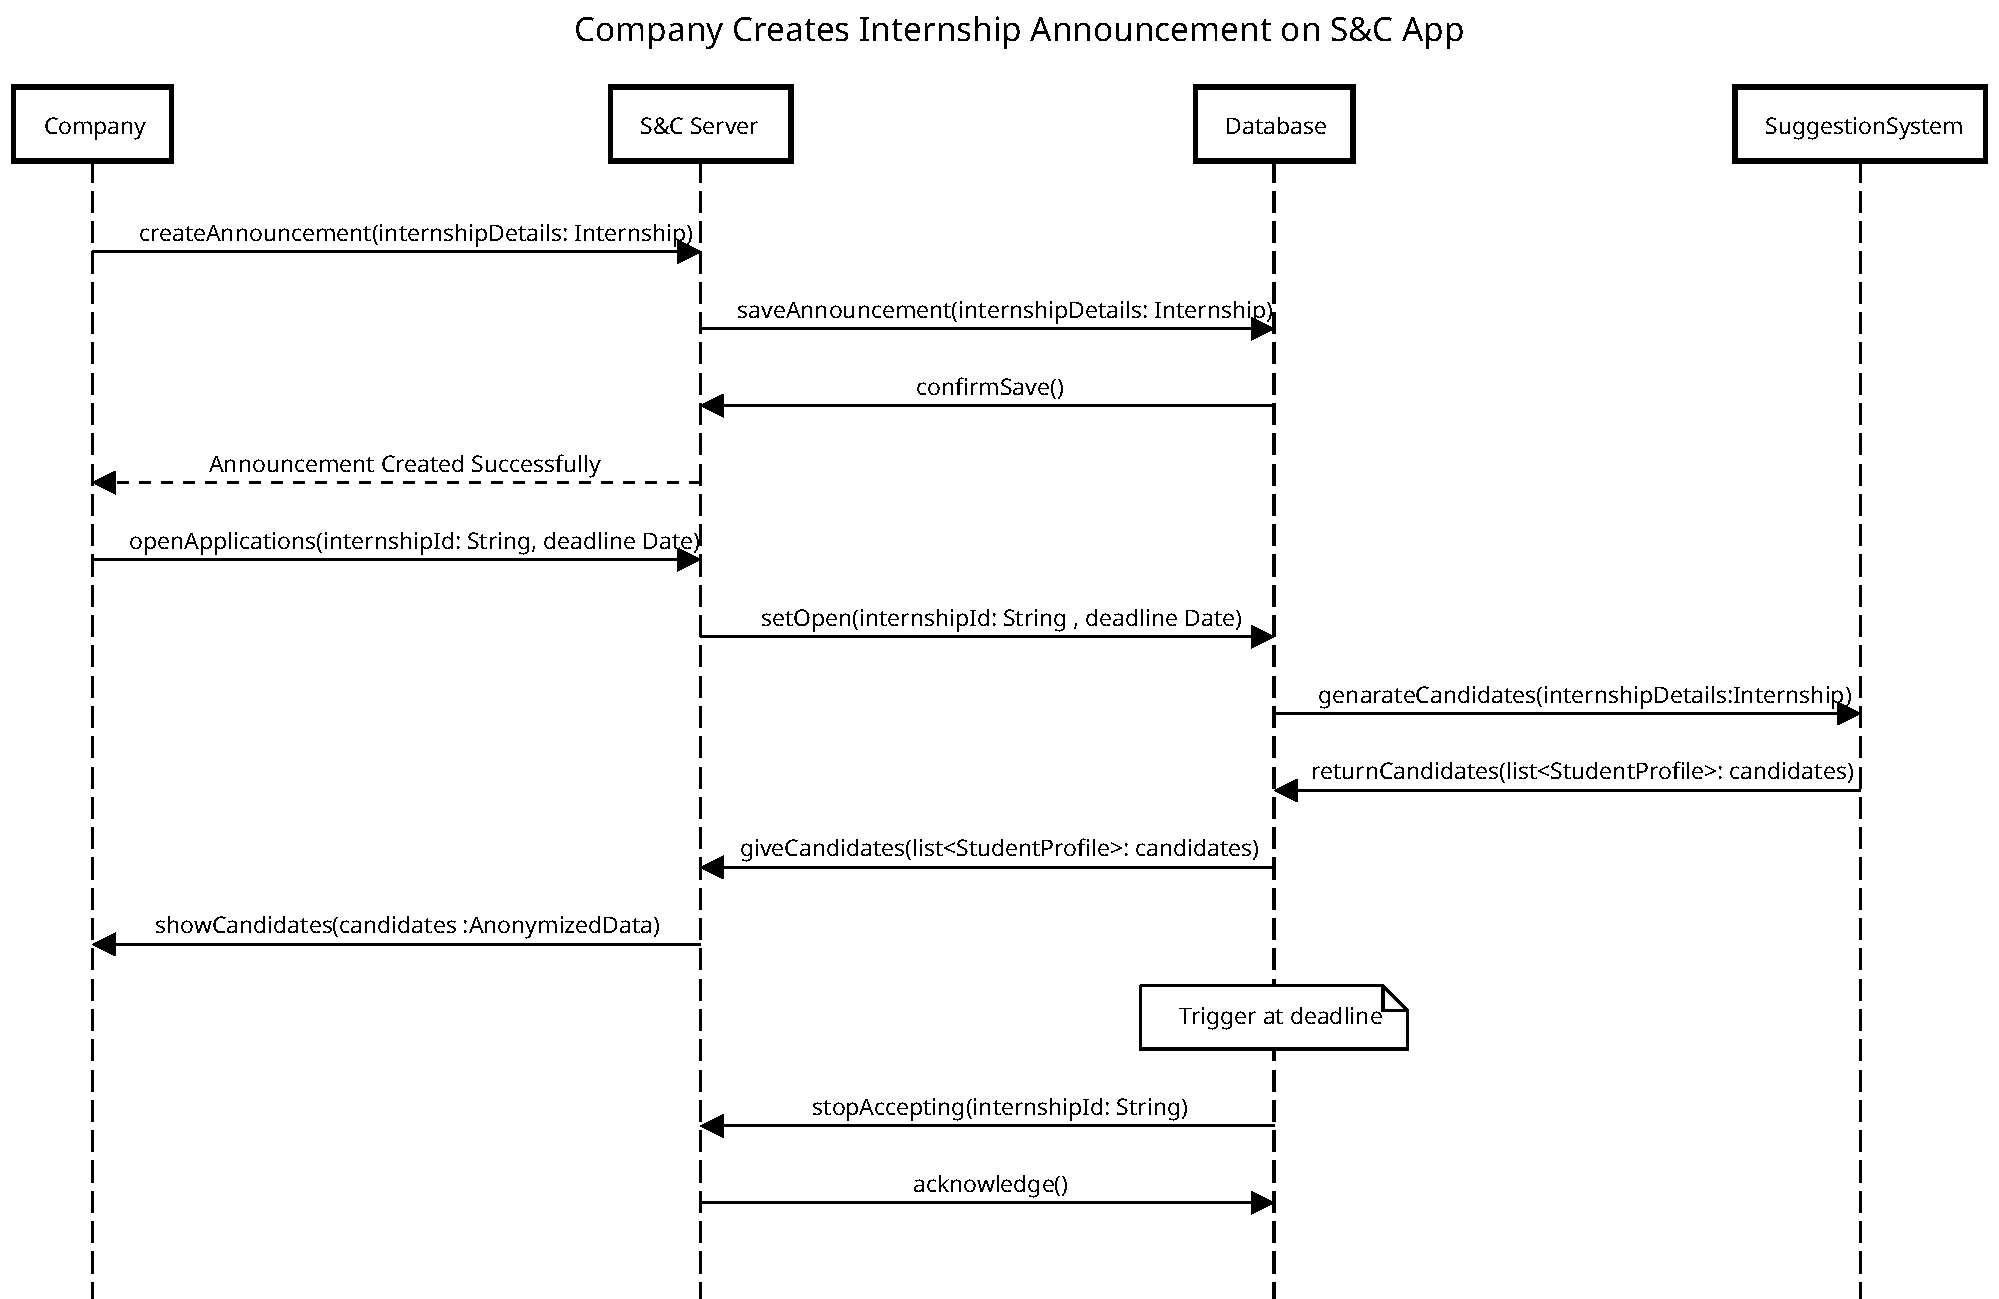
\includegraphics[width=1\textwidth]{Images/UC_9.pdf}
    \caption{Company Creates an Internship Announcement - Use Case Diagram}
    \label{fig:use-case-diagram-9}
\end{figure}

% 10

\subsubsection{UC10: Company looks for extra potential candidates through the recommendation system}
\label{subsubsec:company-looks-for-extra-potential-candidates-through-the-recommendation-system}

\begin{center}
    \begin{longtable}{|l|p{0.75\linewidth}|}
        \hline
        \textbf{Actors:}           & CO, ST                                                                                                                \\
        \hline
        \textbf{Entry Conditions:} & CO is correctly logged in. CO has published an internship listing.                                                    \\
        \hline
        \textbf{Flow of Events:}   & \begin{enumerate}
                                         \item CO visits the "My Internships" page.
                                         \item S\&C fetch the internships from the database.
                                         \item S\&C shows the internships to the CO.
                                         \item CO selects an internship to view the details.
                                         \item S\&C fetch the internship details from the database.
                                         \item S\&C shows the internship details to the CO.
                                         \item CO clicks on the "Applicants" button.
                                         \item S\&C fetch the applicants from the database.
                                         \item S\&C shows the applicants to the CO.
                                         \item CO clicks on "Recommended Candidates" button.
                                         \item (opt. 1) S\&C fetch the recommended candidates from the database.
                                         \item (opt. 2) The list of recommended candidates must be updated.
                                               \begin{enumerate}
                      \item The recommendation system fetches information about the internship.
                      \item The recommendation system computes a set of filters used to find the best candidates.
                      \item The recommendation system fetches the candidates from the database using the filters.
                      \item The recommendation system stores the list of "preferred" candidates in the database.
                  \end{enumerate}
                                         \item S\&C shows the recommended candidates to the CO.
                                         \item CO selects a candidate to view the details of.
                                         \item S\&C fetch the candidate details from the database.
                                         \item S\&C shows the candidate details to the CO.
                                         \item CO, if interested, can "suggests" the internship to the ST by clicking on the "Suggests this Internship" button.
                                         \item S\&C sends the ST a notification email about the internship suggestion.
                                         \item S\&C stores the CO interest for this particular ST.
                                     \end{enumerate} \\
        \hline
        \textbf{Exit Conditions:}  & CO has increased the number of potential candidates for the internship.                                               \\
        \hline
        \textbf{Exceptions:}       & S\&C generated an internal error.                                                                                     \\
        \hline
    \end{longtable}
\end{center}

\begin{figure}
    \centering
    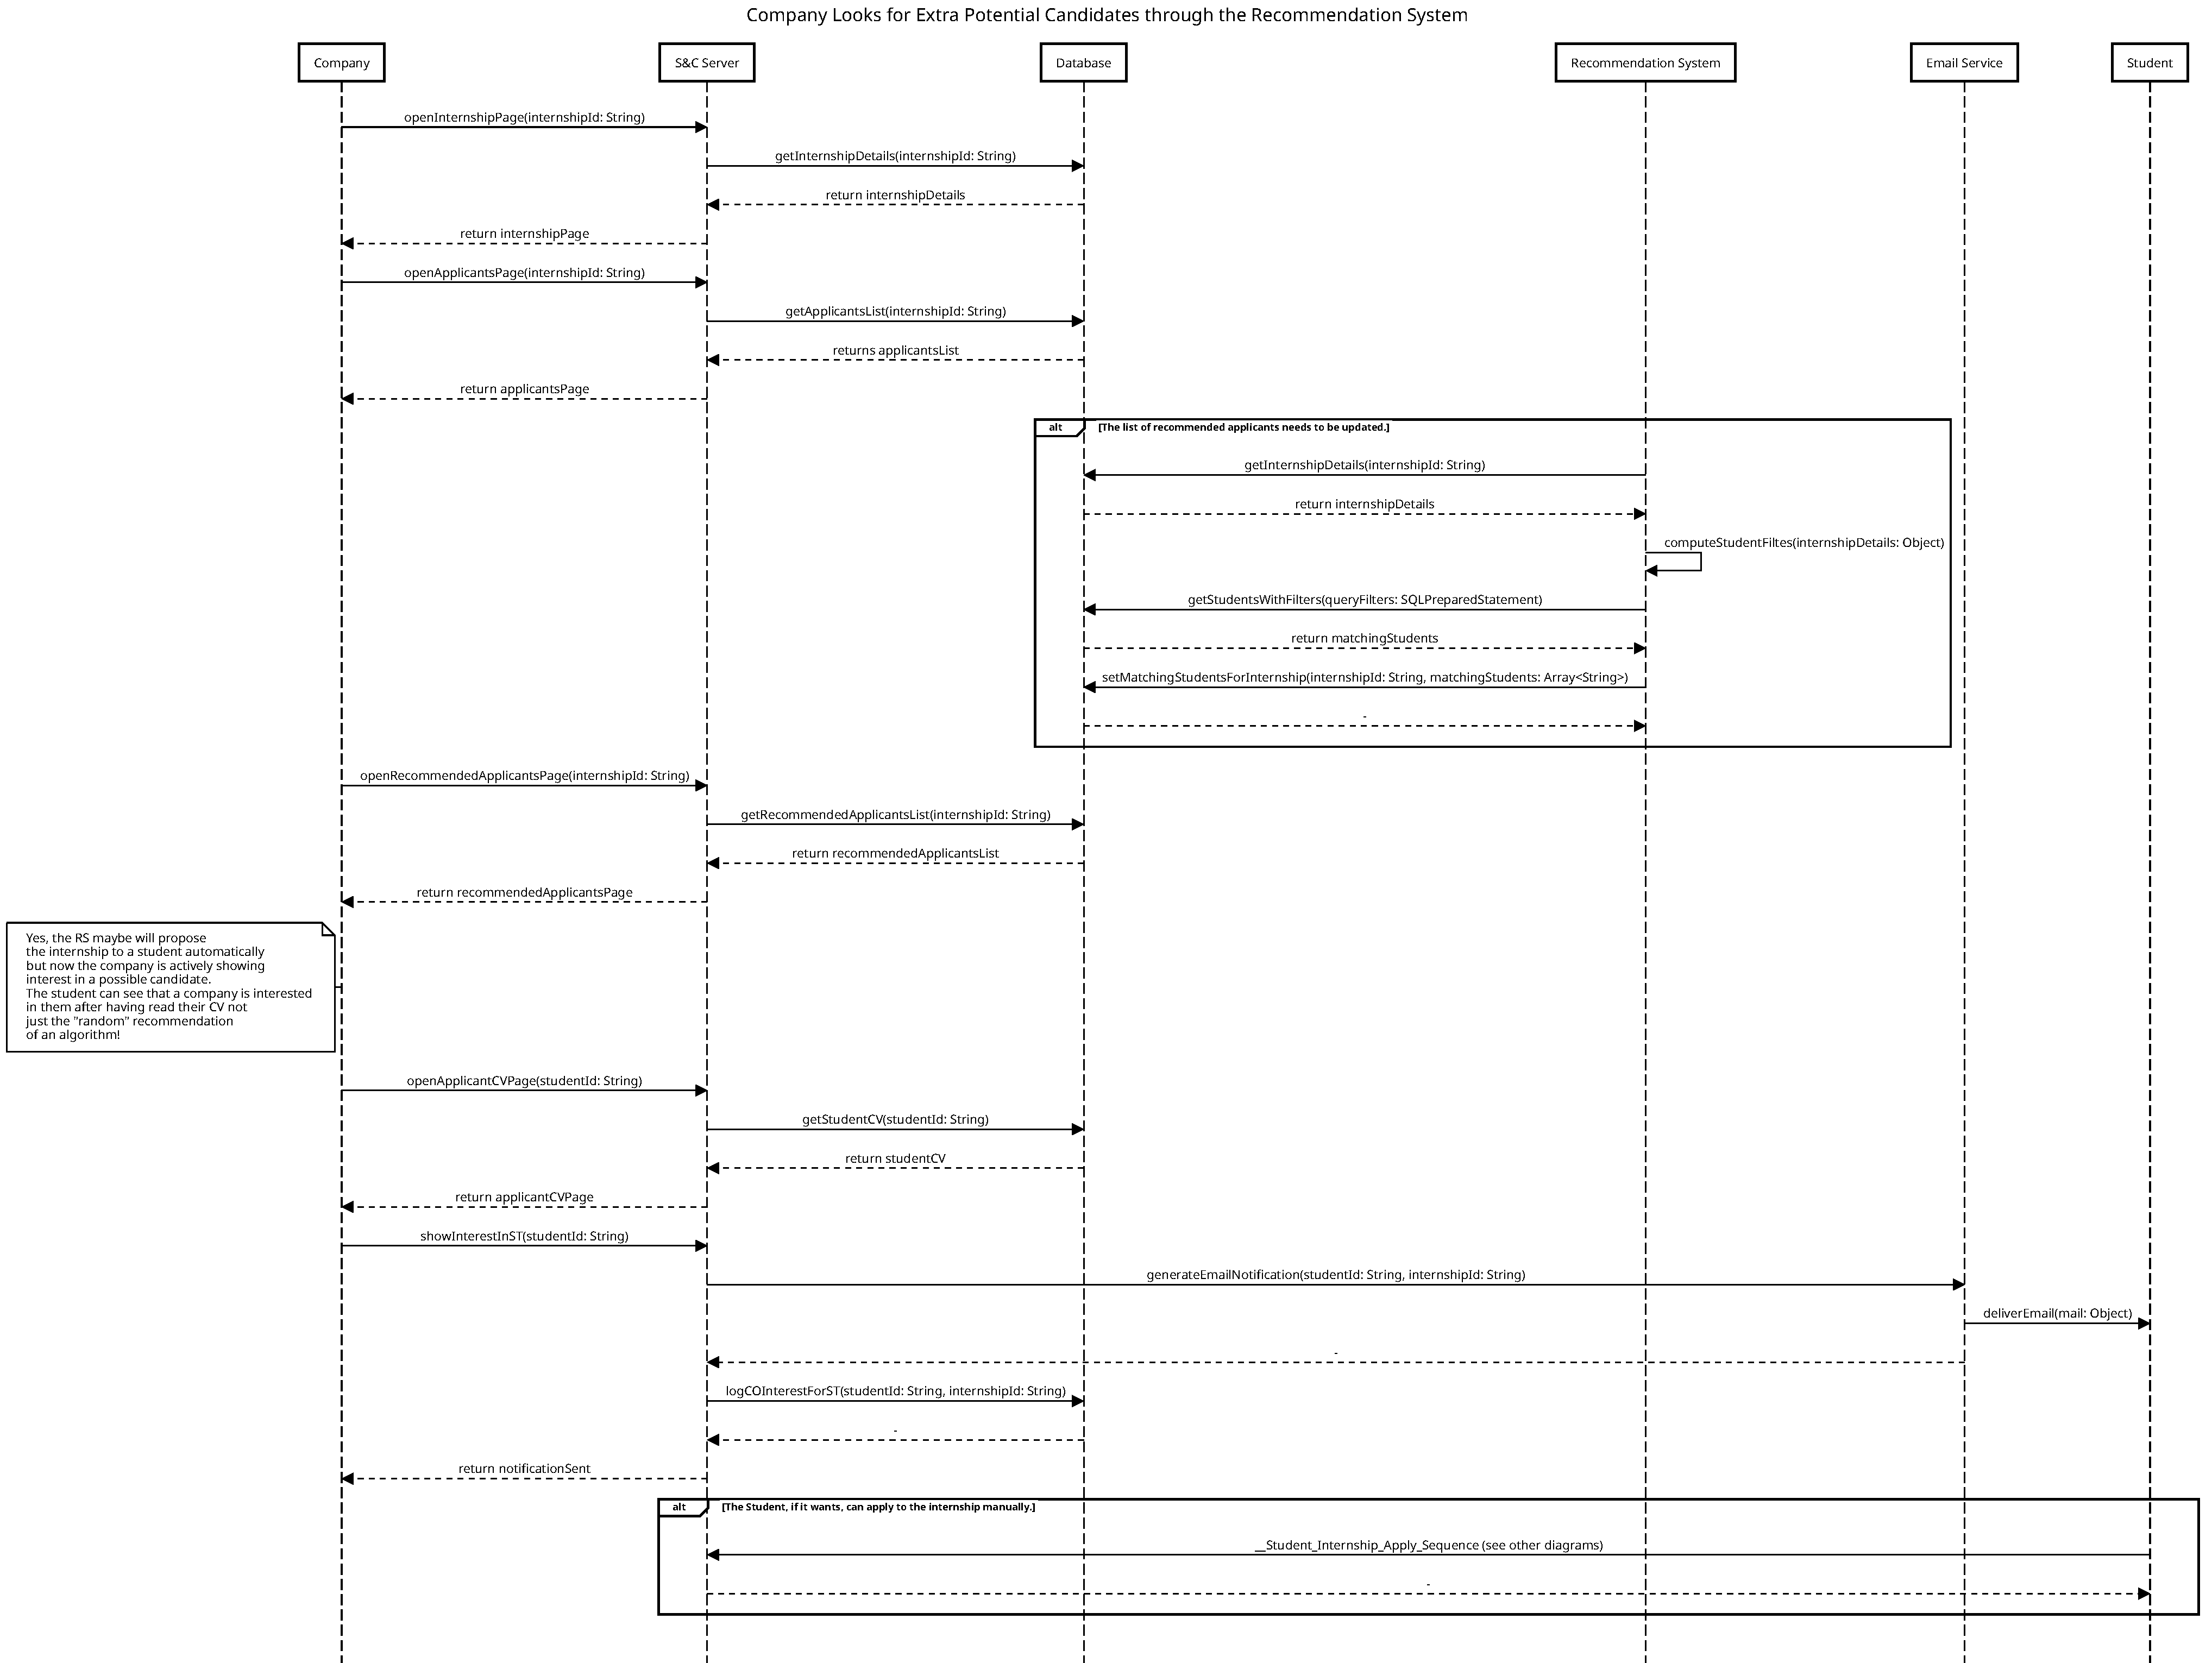
\includegraphics[width=1.0\textwidth]{Images/UC_10.pdf}
    \caption{Company Looks for Extra Potential Candidates through the Recommendation System - Use Case Diagram}
    \label{fig:use-case-diagram-10}
\end{figure}

% 11

\subsubsection{UC11: Company creates a questionnaire for the applicants}
\label{subsubsec:company-creates-a-questionnaire-for-the-applicants}

\begin{center}
    \begin{longtable}{|l|p{0.75\linewidth}|}
        \hline
        \textbf{Actors:}           & CO                                                                                                        \\
        \hline
        \textbf{Entry conditions:} & CO is correctly logged in. An internship has reached the deadline and now has to evaluate the candidates. \\                                                                                                  \\
        \hline
        \textbf{Flow of Events:}   & \begin{enumerate}
                                         \item CO visits the "My Internships" page.
                                         \item S\&C fetch the internships from the database.
                                         \item S\&C shows the internships to the CO.
                                         \item CO selects an internship to view the details.
                                         \item S\&C fetch the internship details from the database.
                                         \item S\&C shows the internship details to the CO.
                                         \item CO clicks on the "Create Questionnaire" button.
                                         \item S\&C sends the questionnaire template to the CO.
                                         \item CO fills the questionnaire  with relevant questions.
                                         \item S\&C stores the questionnaire in the database.
                                         \item S\&C notifies the CO that the questionnaire was successfully created.
                                     \end{enumerate}                                \\
        \hline
        \textbf{Exit Conditions:}  & CO has successfully created a questionnaire for the applicants or a partial version has been saved.       \\
        \hline
        \textbf{Exceptions:}       & S\&C generated an internal error.                                                                         \\
        \hline
    \end{longtable}
\end{center}

\begin{figure}[H]
    \centering
    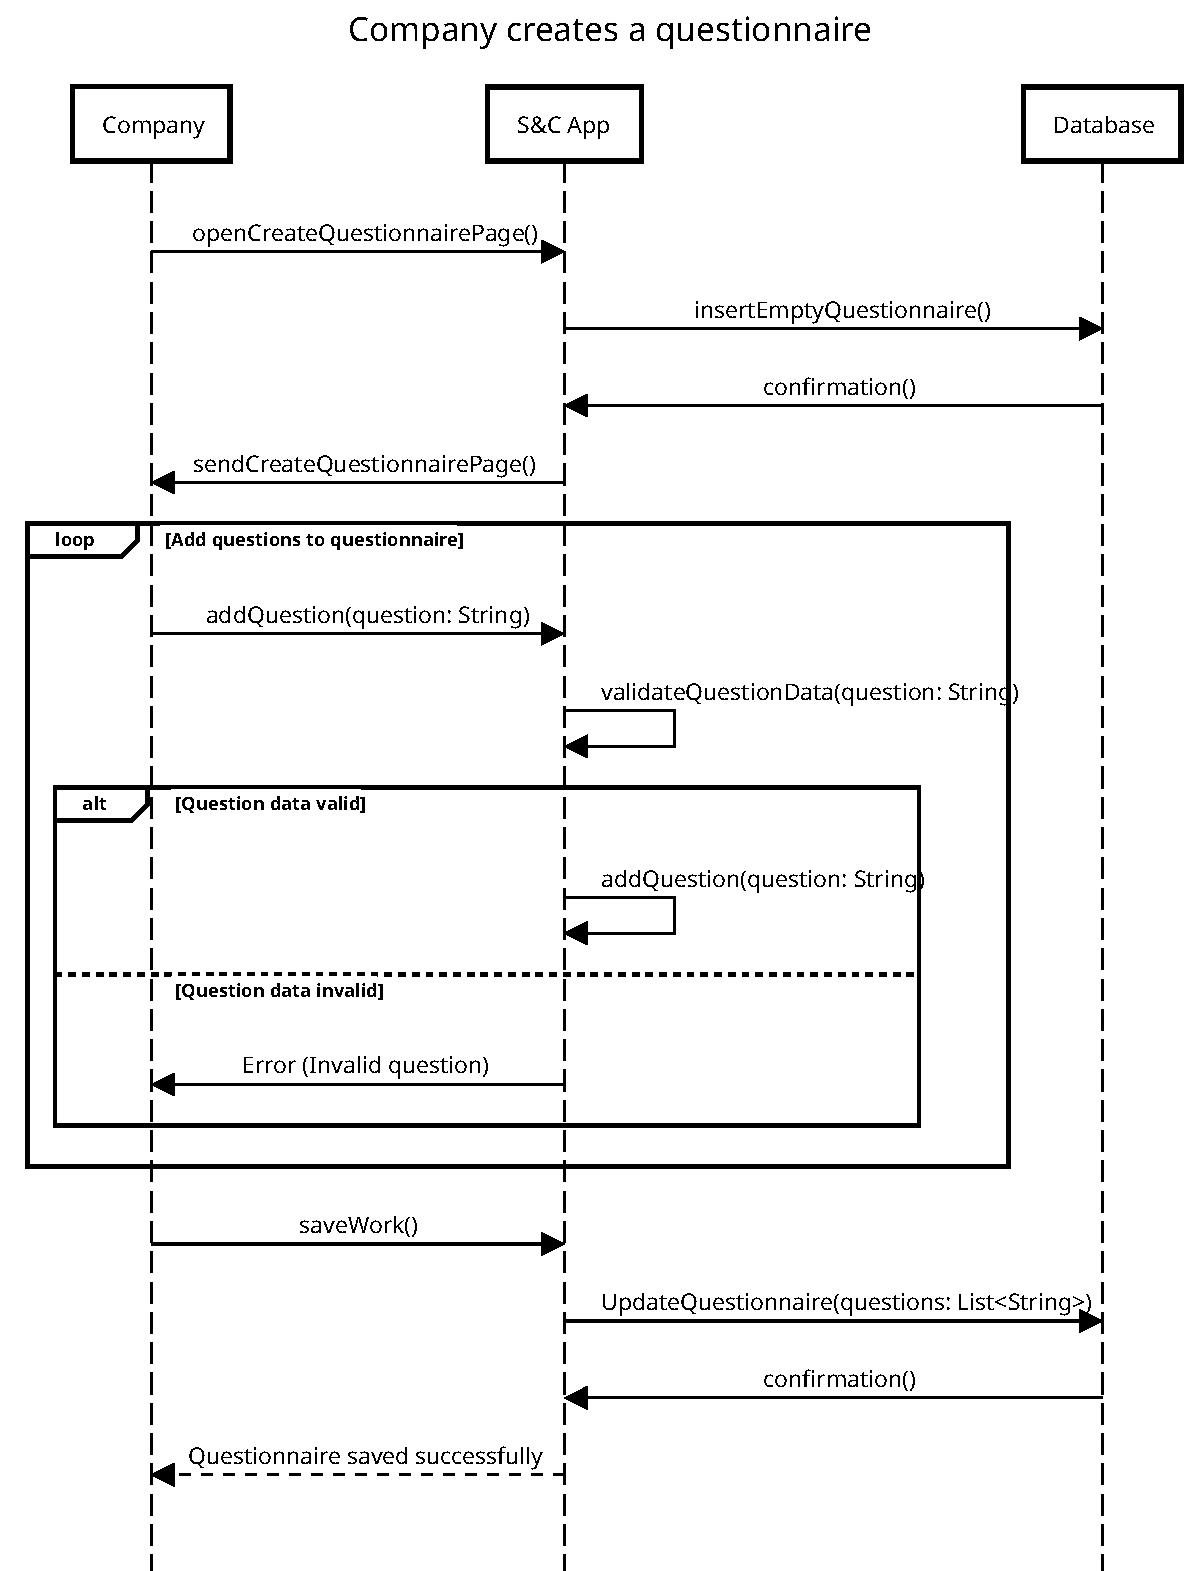
\includegraphics[width=1\textwidth]{Images/UC_11.pdf}
    \caption{Company Creates a Questionnaire for the Applicants - Use Case Diagram}
    \label{fig:use-case-diagram-11}
\end{figure}

% 12

\subsubsection{UC12: Company selects applicant student for its internship}
\label{subsubsec:company-select-applicant-student-for-its-internship}

\begin{center}
    \begin{longtable}{|l|p{0.75\linewidth}|}
        \hline
        \textbf{Actors:}           & CO                                                                                                                      \\
        \hline
        \textbf{Entry Conditions:} & CO is correctly logged in, has already created an internship listing, and has received applications from STs.
        CO has already loaded the questionnaire for the STs.CO is correctly logged in. CO has published an internship listing.                               \\
        \hline
        \textbf{Flow of Events:}   & \begin{enumerate}
                                         \item CO request the page that shows the applications for his internship.
                                         \item S\&C fetches the applications from the database.
                                         \item S\&C shows the applications to the CO.
                                         \item CO selects the STs he wants to send the questionnaire.
                                         \item S\&C store the selection of STs linked to the internship.
                                         \item CO confirm the questionnaire to be sent to the selected STs.
                                         \item S\&C notifies the selected STs that they have a questionnaire to fill, inherent to the CO's internship, via email.
                                     \end{enumerate} \\
        \hline
        \textbf{Exit Conditions:}  & CO receives a confirmation that S\&C has sent the questionnaire to the selected STs.                                    \\
        \hline
        \textbf{Exceptions:}       & S\&C generated an internal error.                                                                                       \\
        \hline
    \end{longtable}
\end{center}

\begin{figure}[H]
    \centering
    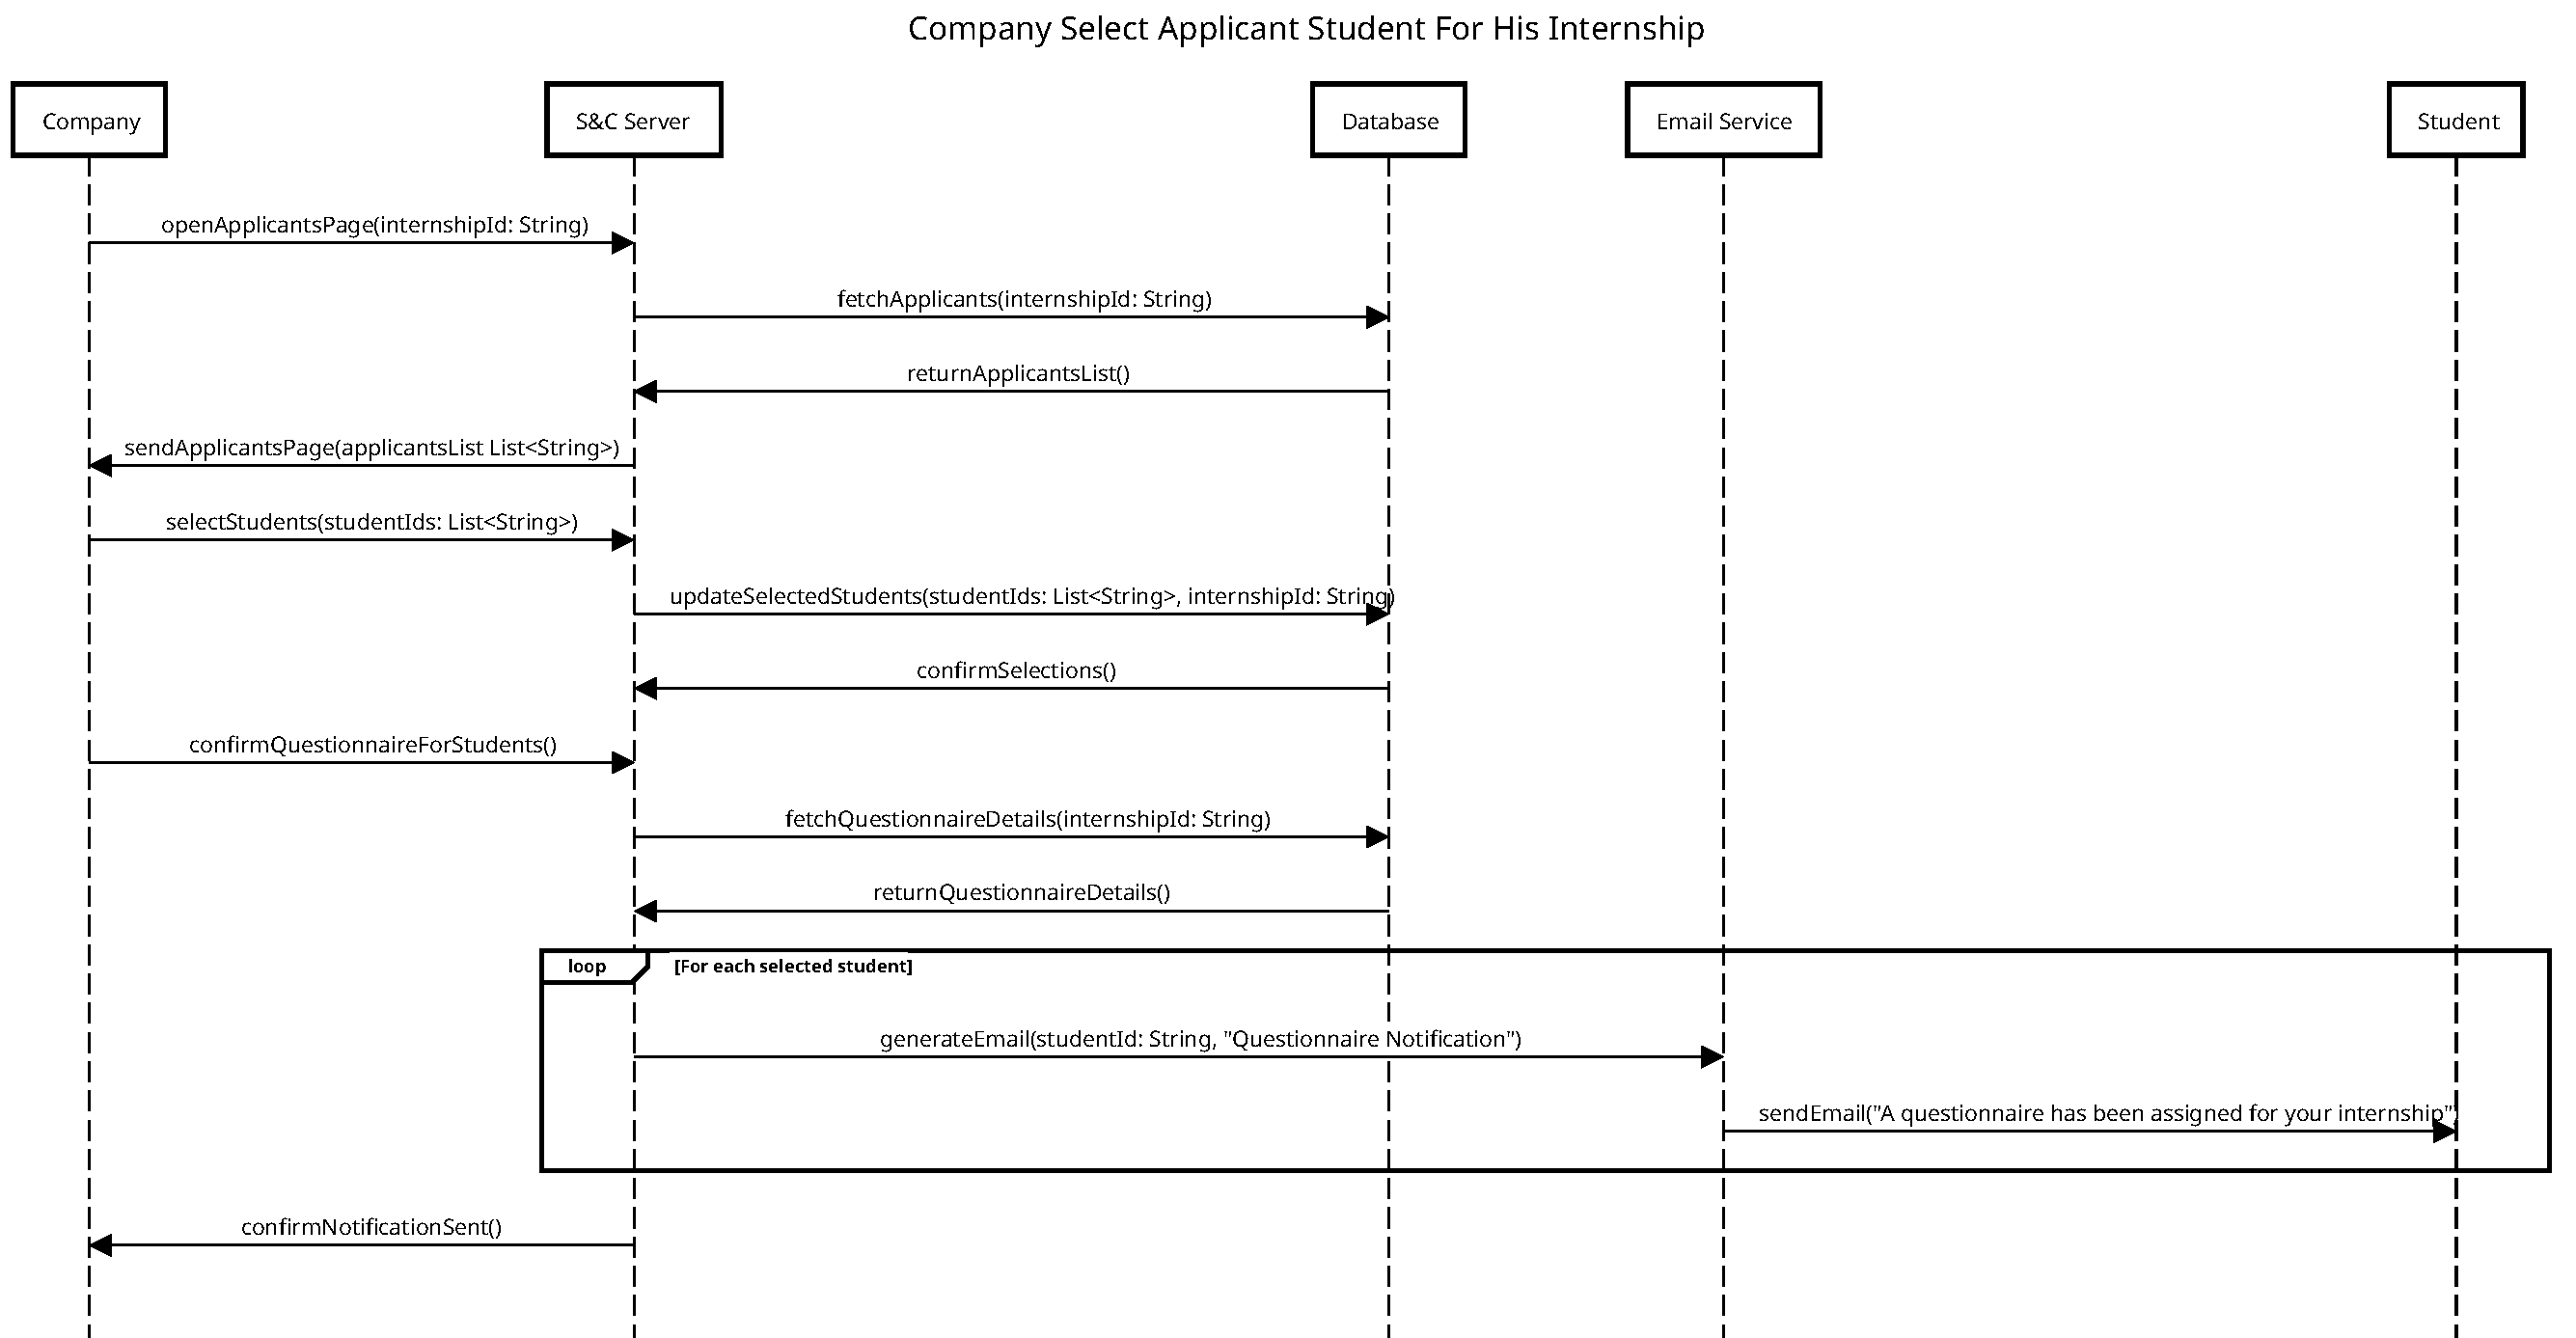
\includegraphics[width=1\textwidth]{Images/UC_12.pdf}
    \caption{Company Selects Applicant Student for its Internship - Use Case Diagram}
    \label{fig:use-case-diagram-12}
\end{figure}

% 13

\subsubsection{UC13: Company creates a complaints}
\label{subsubsec:company-creates-a-complaints}

\begin{center}
    \begin{longtable}{|l|p{0.75\linewidth}|}
        \hline
        \textbf{Actors:}           & CO, (opt) UN                                                                                                                     \\
        \hline
        \textbf{Entry Conditions:} & CO is correctly logged in. CO had decided to create a complaint about the internship it's holding.                               \\
        \hline
        \textbf{Flow of Events:}   & \begin{enumerate}
                                         \item CO clicks on the "Create Complaint" button.
                                         \item S\&C send to the CO a form to fill with the complaint details.
                                         \item CO fills the form and submits it.
                                         \item S\&C stores the complaint in the database.
                                         \item S\&C request to the Emailing system to send an email to the UN about a new complaint about an internship of one of it's ST.
                                         \item The Emailing system sends the email to the UN.
                                         \item S\&C notifies the CO that the complaint was successfully submitted.
                                         \item (opt) UN acknowledges the complaint.
                                         \item (opt) S\&C change the status of the complaint to "Acknowledged".
                                     \end{enumerate} \\
        \hline
        \textbf{Exit Conditions:}  & CO has increased the number of potential candidates for the internship.                                                          \\
        \hline
        \textbf{Exceptions:}       & S\&C generated an internal error.                                                                                                \\
        \hline
    \end{longtable}
\end{center}

\begin{figure}[H]
    \centering
    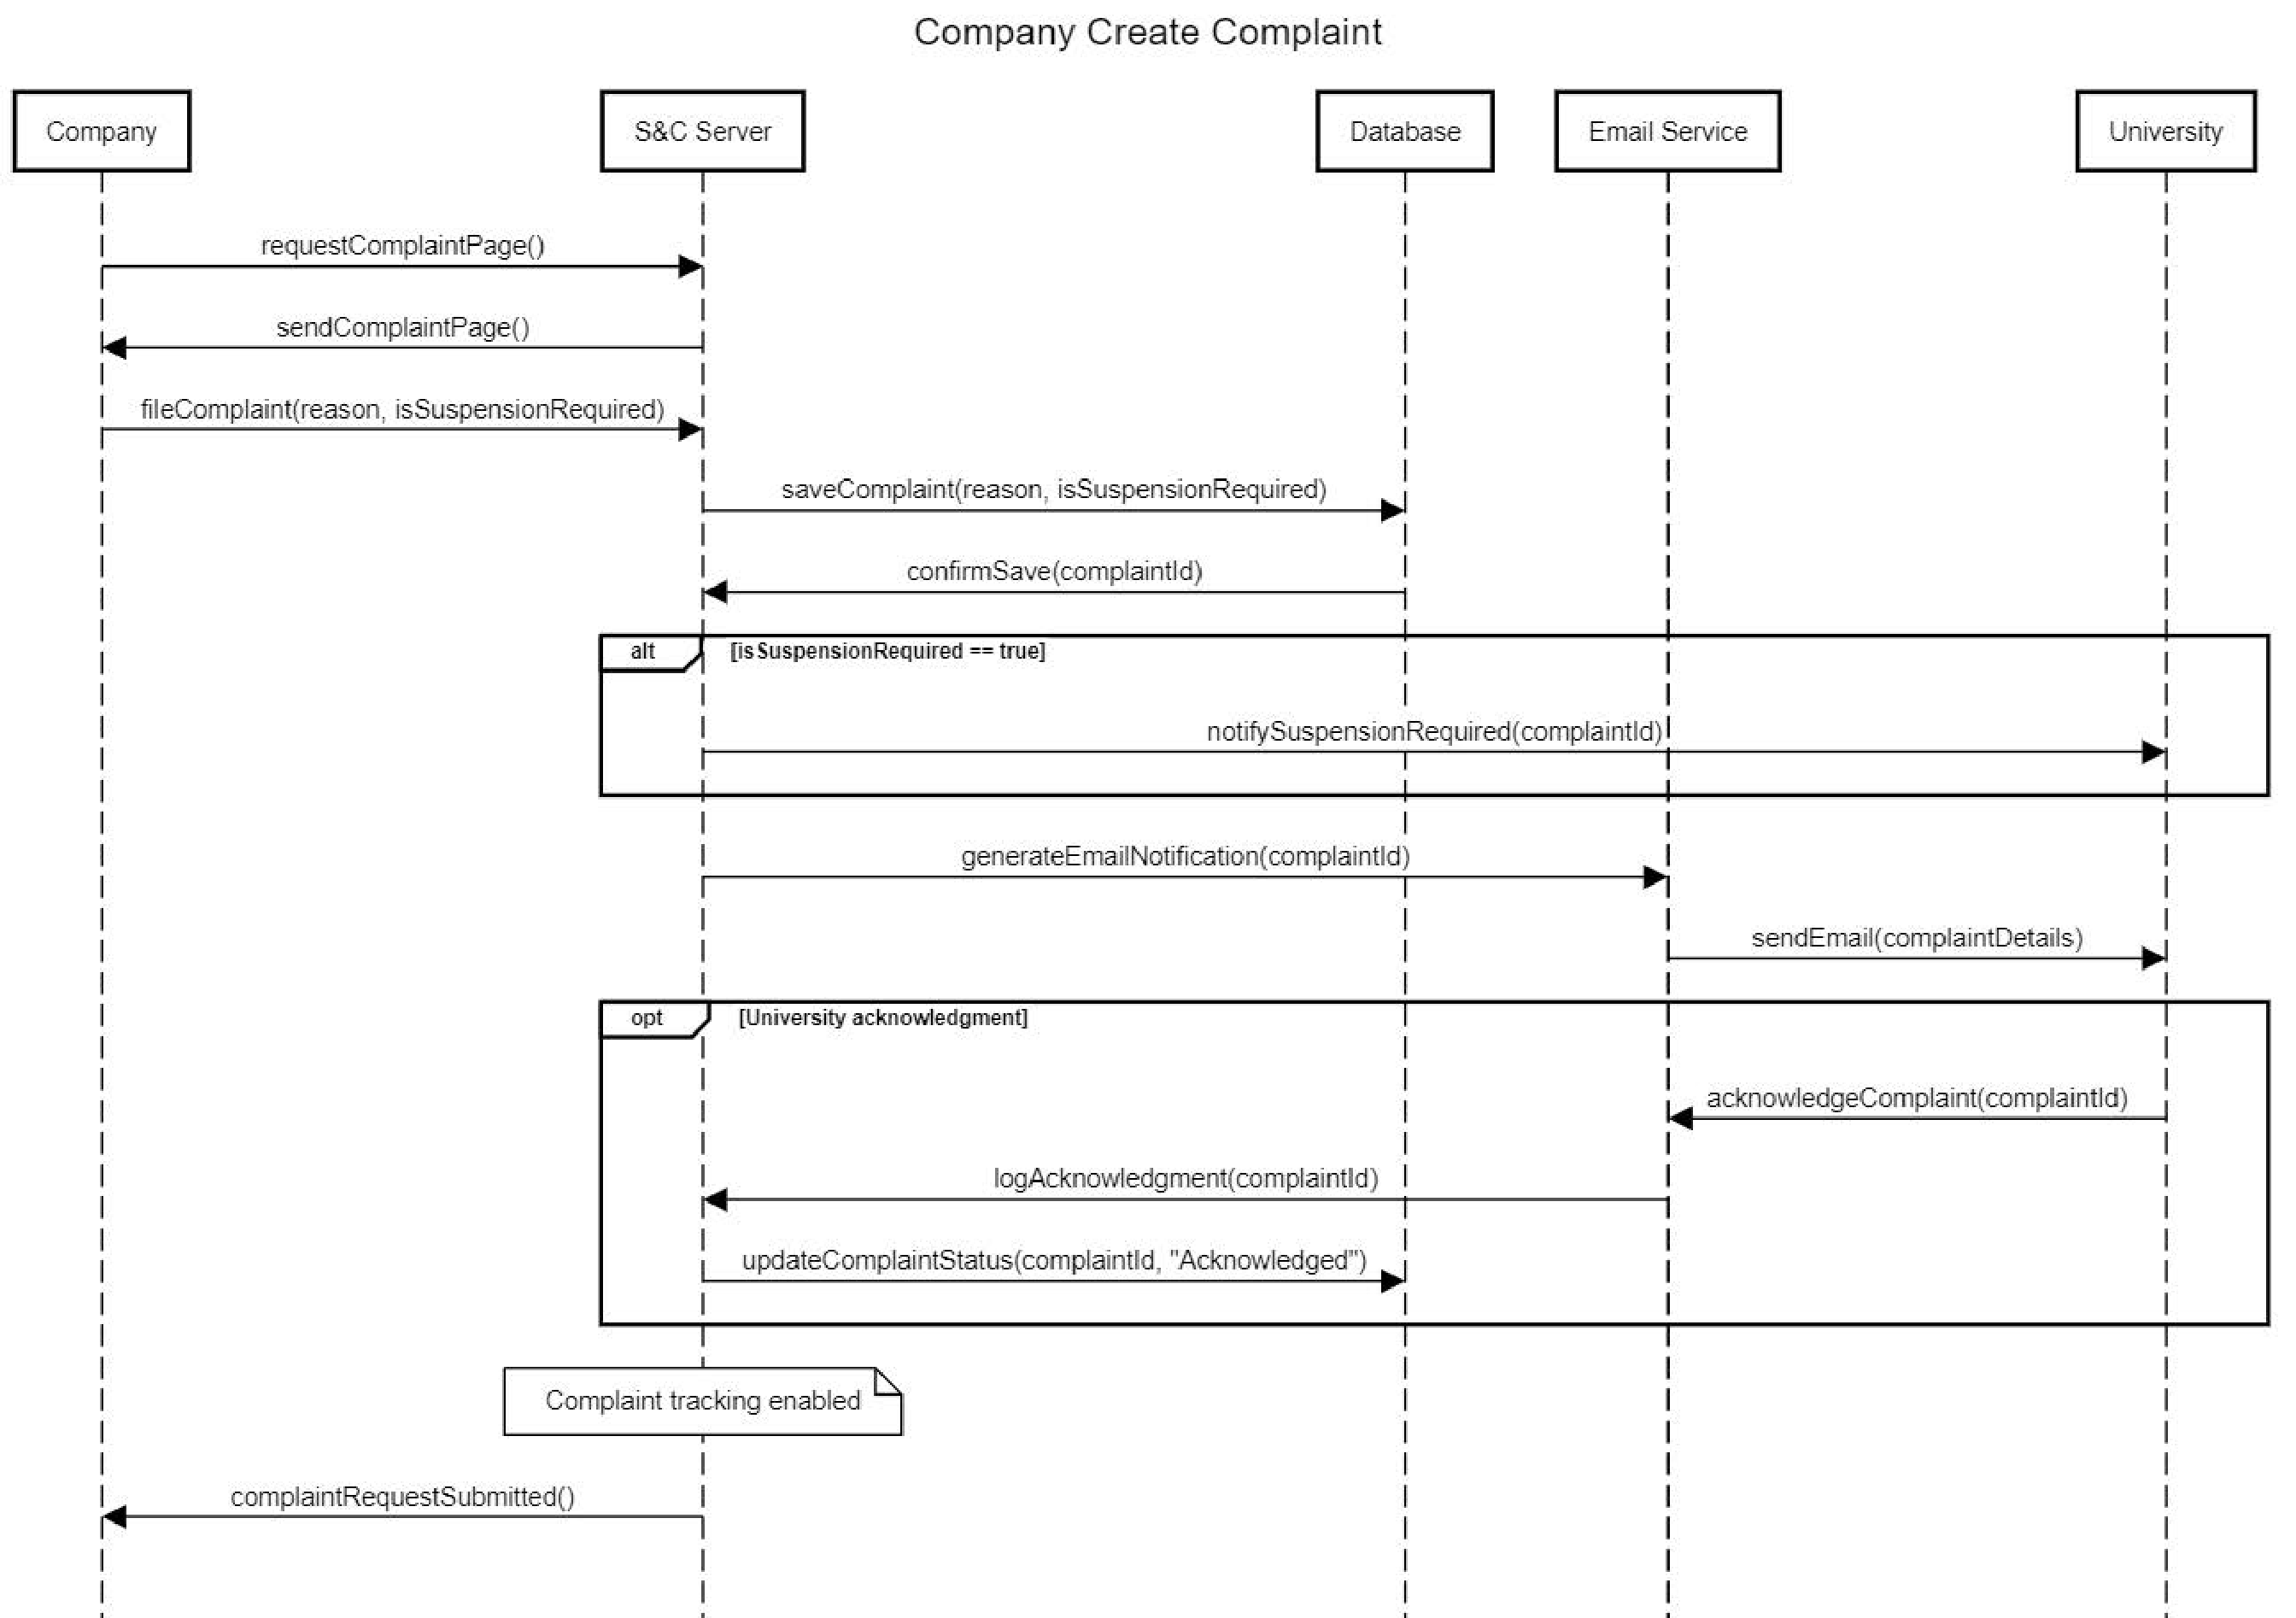
\includegraphics[width=1.0\textwidth]{Images/UC_13.pdf}
    \caption{Company Creates a Complaint - Use Case Diagram}
    \label{fig:use-case-diagram-13}
\end{figure}

% 14

\subsubsection{UC14: Company answers questionnaire at internship completion}
\label{subsubsec:company-answers-questionnaire-at-internship-completion}

\begin{center}
    \begin{longtable}{|l|p{0.75\linewidth}|}
        \hline
        \textbf{Actors:}           & CO                                                                                                                                                        \\
        \hline
        \textbf{Entry Conditions:} & CO is correctly logged in. The internship has ended. CO has received a notification to fill the questionnaire.                                            \\
        \hline
        \textbf{Flow of Events:}   & \begin{enumerate}
                                         \item CO clicks on the "Fill Questionnaire" button.
                                         \item S\&C fetch the questionnaire from the database.
                                         \item S\&C shows the questionnaire to the CO.
                                         \item CO fills each question and submits it.
                                         \item S\&C stores the questionnaire in the database.
                                         \item S\&C notifies the UN that the questionnaire was successfully submitted.
                                         \item S\&C feeds the answers of the questionnaire to the suggestion system to improve it's response on how to improve a CV or an internship advertisement.
                                     \end{enumerate} \\
        \hline
        \textbf{Exit Conditions:}  & CO receive the confirmation of the questionnaire being saved correctly                                                                                    \\
        \hline
        \textbf{Exceptions:}       & S\&C generated an internal error.                                                                                                                         \\
        \hline
    \end{longtable}
\end{center}

\begin{figure}[H]
    \centering
    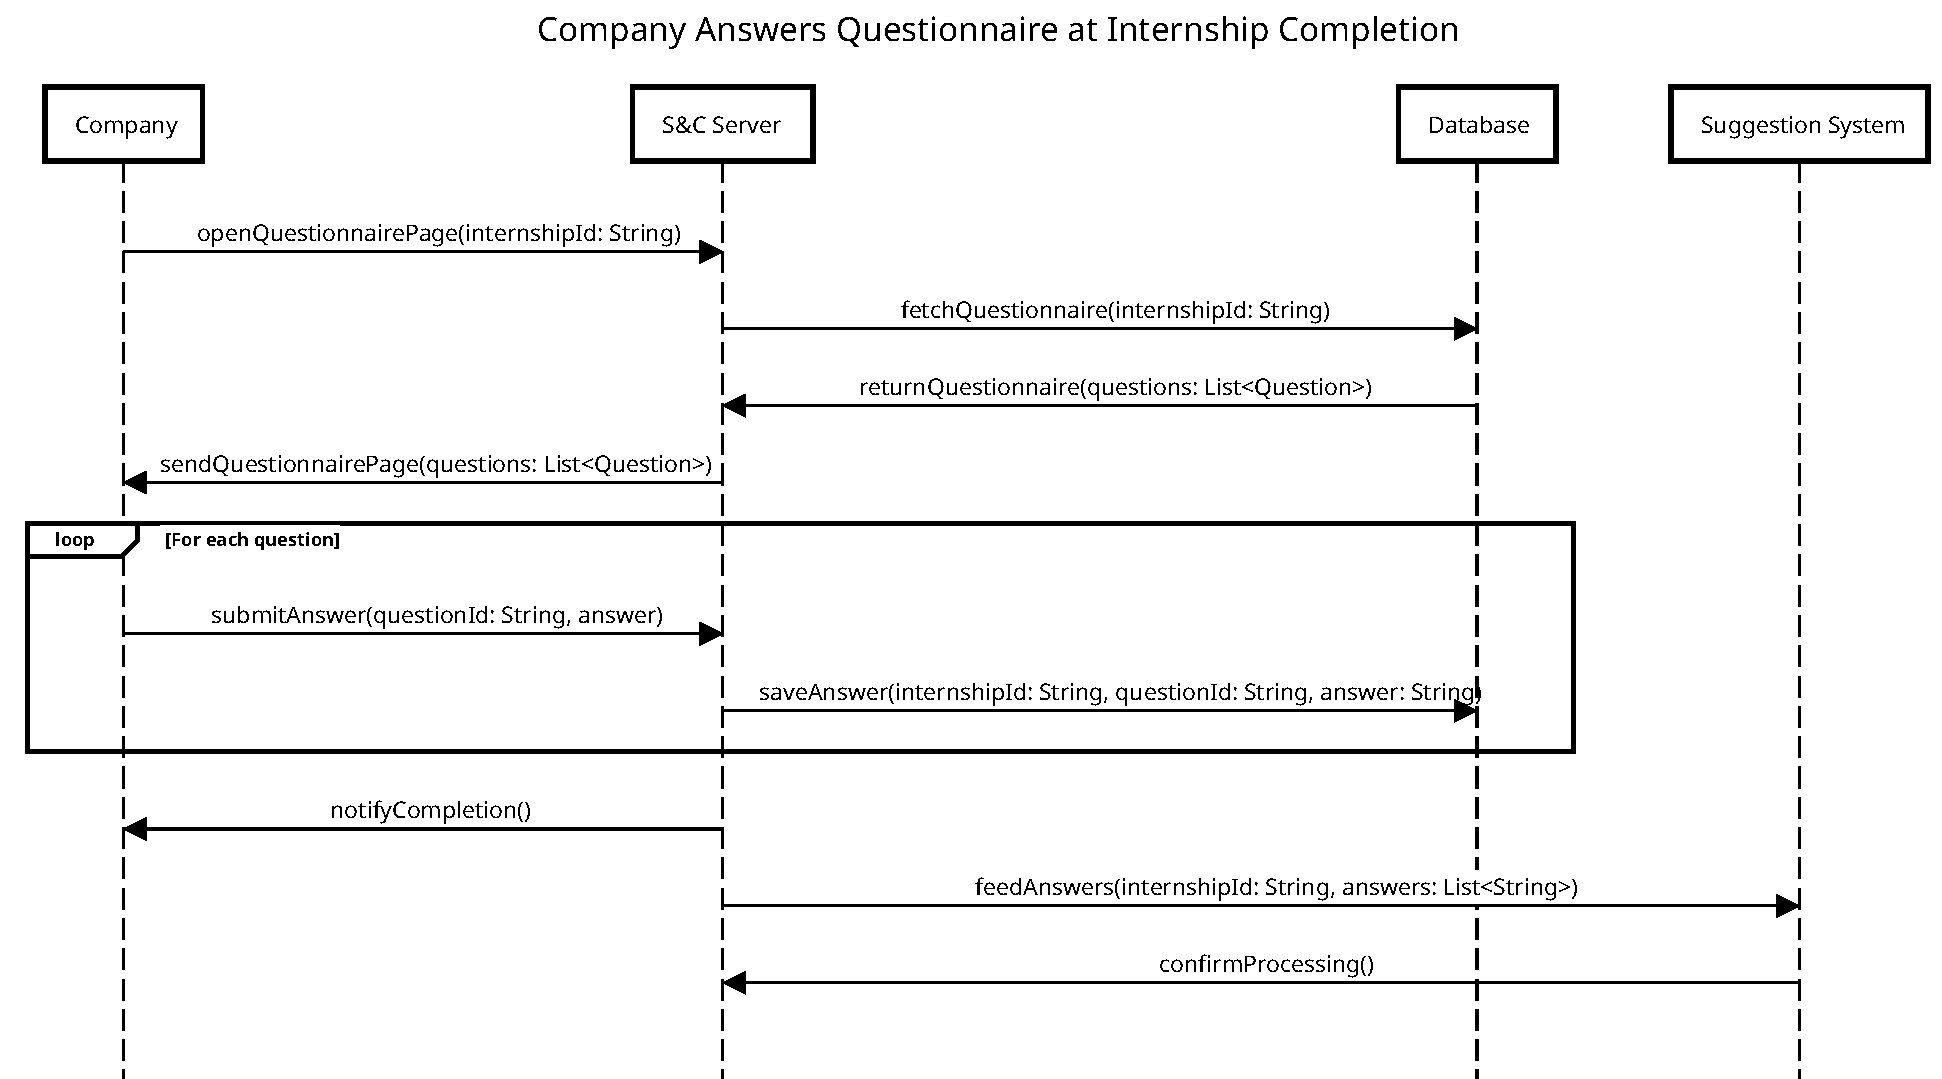
\includegraphics[width=1.0\textwidth]{Images/UC_14.pdf}
    \caption{Company Answers Questionnaire at Internship Completion - Use Case Diagram}
    \label{fig:use-case-diagram-14}
\end{figure}

% 15

\subsubsection{UC15: Company decides who to hire for an internship}
\label{subsubsec:company-decides-who-to-hire-for-an-internship}

\begin{center}
    \begin{longtable}{|l|p{0.75\linewidth}|}
        \hline
        \textbf{Actors:}           & CO, ST                                                                                  \\
        \hline
        \textbf{Entry Conditions:} & CO is correctly logged in. CO has published an internship listing.                      \\
        \hline
        \textbf{Flow of Events:}   & \begin{enumerate}
                                         \item CO selects an internship to view the details of.
                                         \item S\&C fetch the internship details from the database.
                                         \item S\&C shows the internship details to the CO.
                                         \item CO clicks on the "Applicants" button.
                                         \item S\&C fetch the applicants from the database.
                                         \item S\&C shows the applicants to the CO.
                                         \item CO selects "Show Questionnaires Results" button.
                                         \item S\&C fetch the questionnaires results from the database.
                                         \item S\&C shows the questionnaires results to the CO.
                                         \item CO evaluates the candidates profiles:
                                               \begin{enumerate}
                      \item CO clicks on the "Details" button next to a candidate.
                      \item S\&C fetch the candidate details from the database.
                      \item S\&C fetch the candidate questionnaire answers from the database.
                      \item S\&C shows the candidate details and questionnaire answers to the CO.
                  \end{enumerate}
                                         \item CO decides who to interview and contacts them. At the end, CO decides who to hire.
                                         \item CO clicks on the "Hire" button next to the candidate.
                                         \item S\&C stores the hiring decision in the database.
                                         \item S\&C changes the status of the internship to "On-Going".
                                     \end{enumerate} \\
        \hline
        \textbf{Exit Conditions:}  & CO has successfully hired a candidate for the internship.                               \\
        \hline
        \textbf{Exceptions:}       & S\&C generated an internal error.                                                       \\
        \hline
    \end{longtable}
\end{center}

\begin{figure}[H]
    \centering
    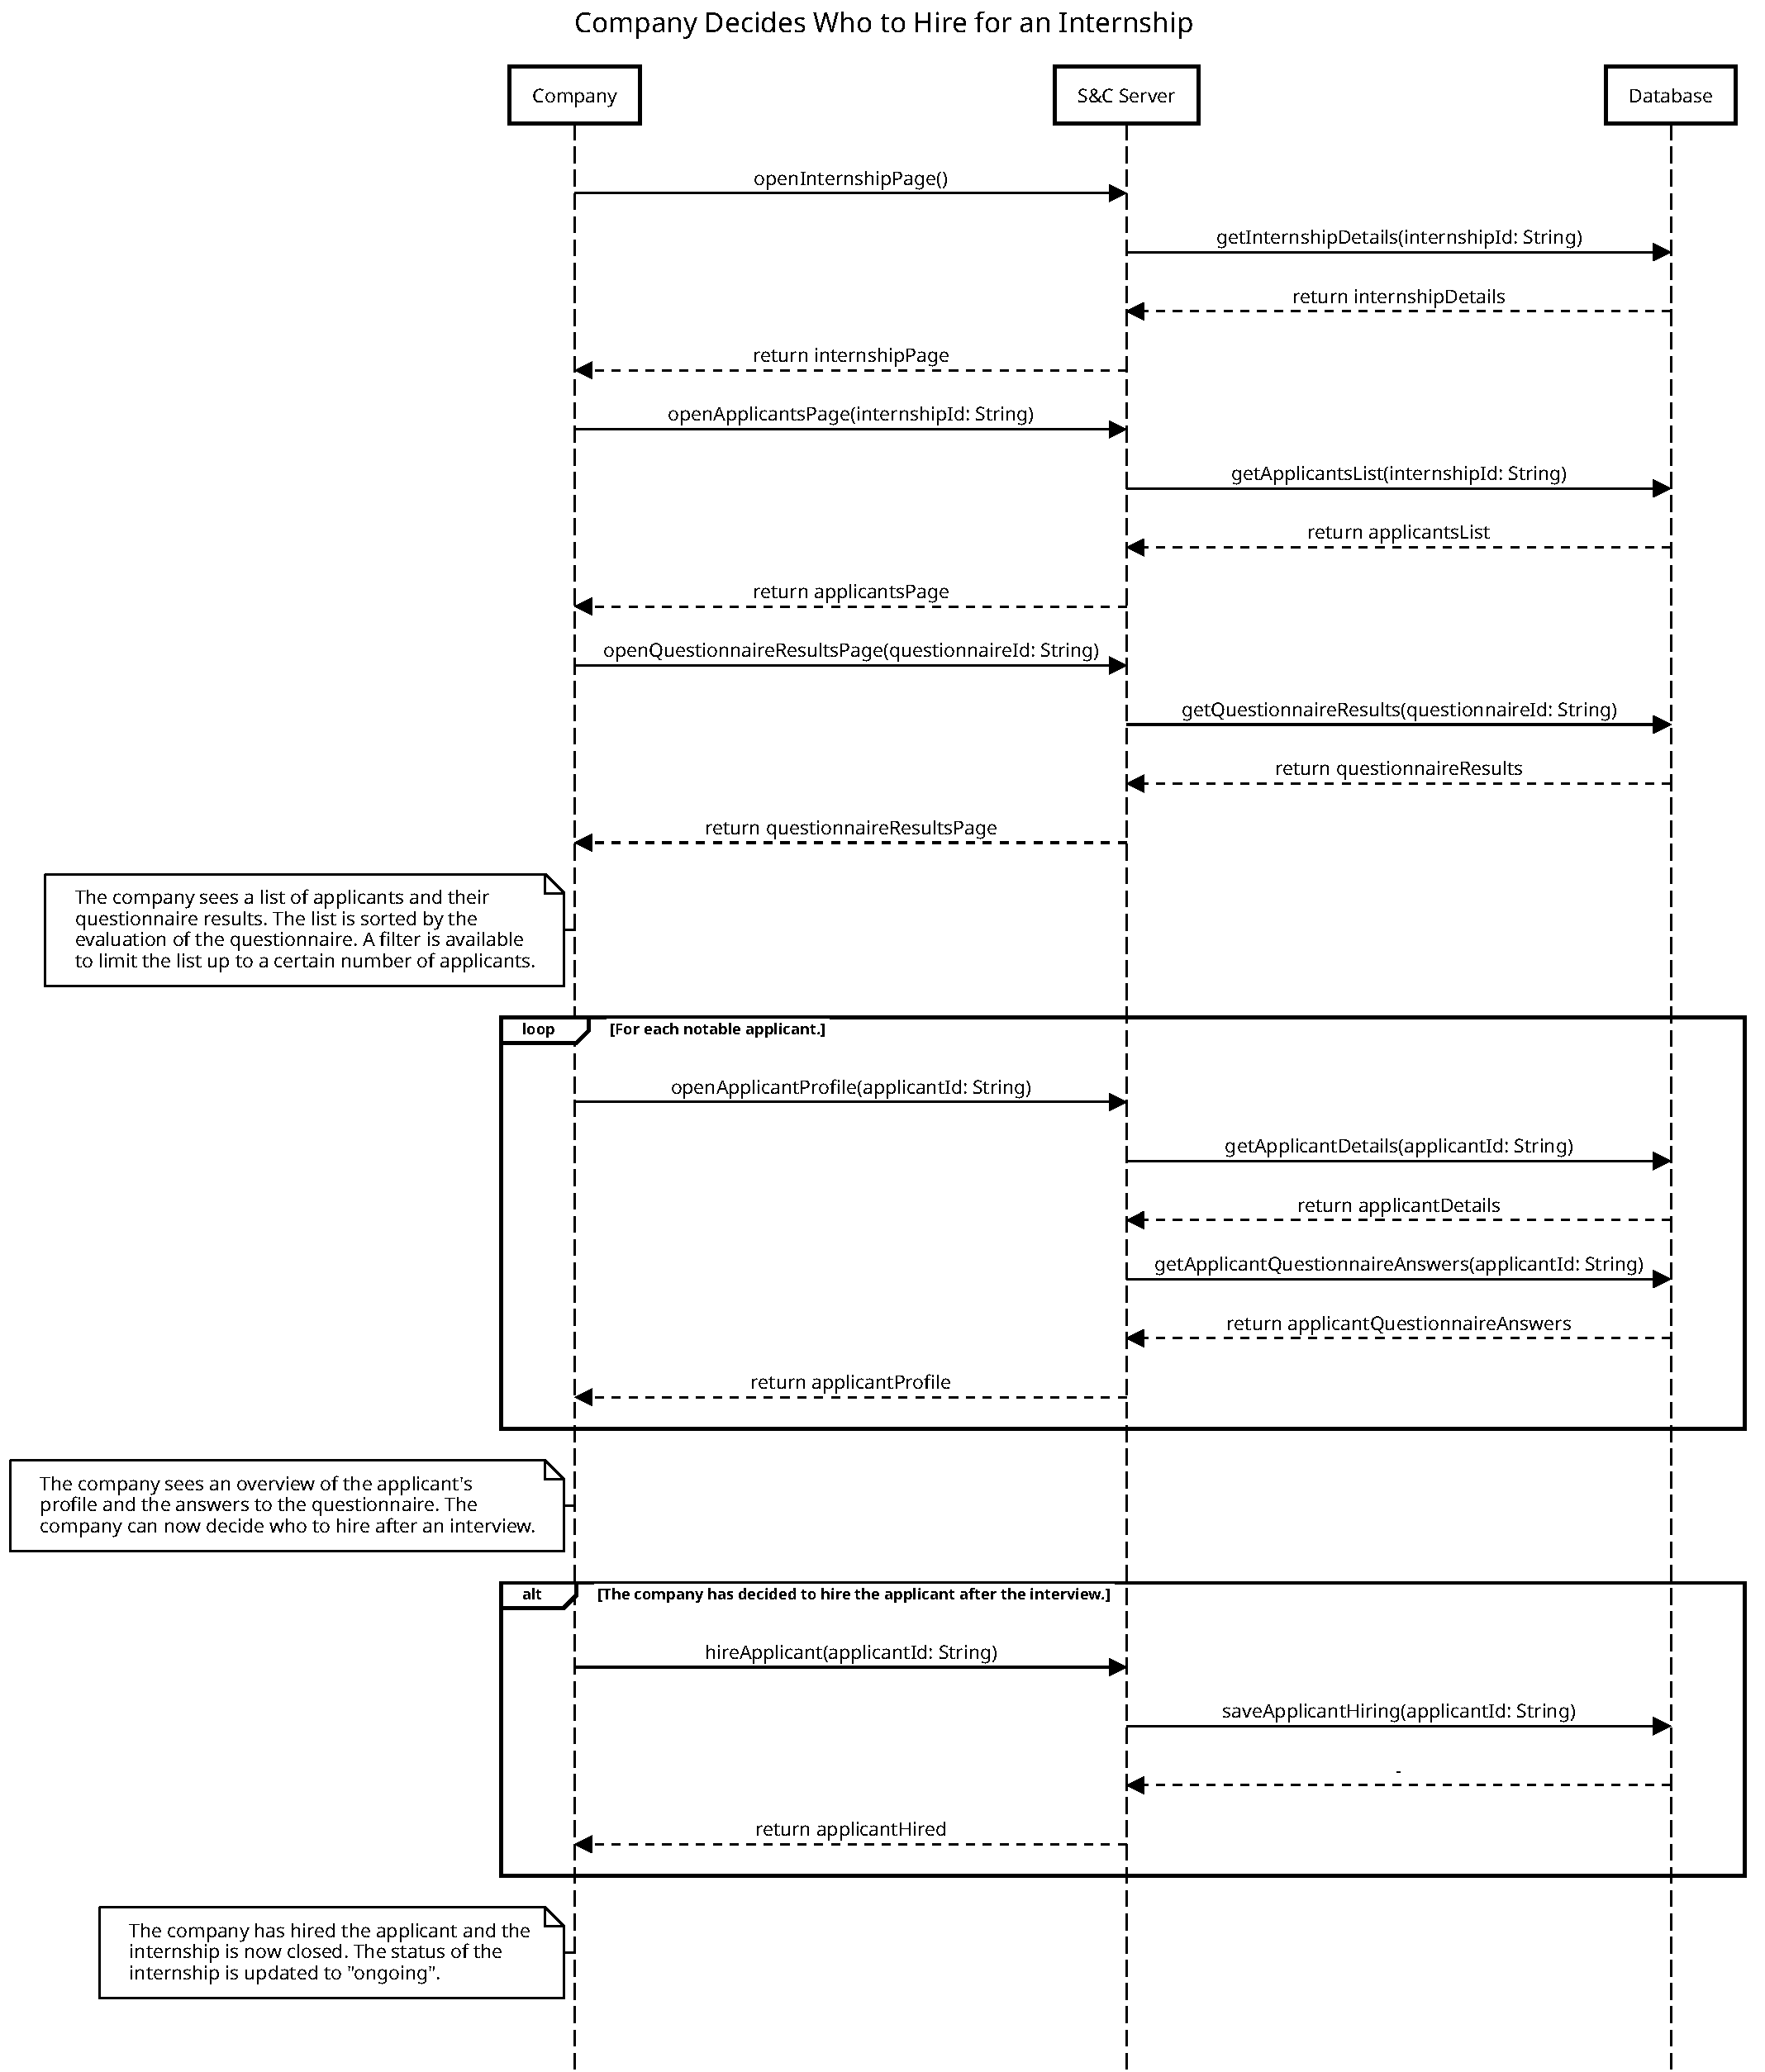
\includegraphics[width=1.0\textwidth]{Images/UC_14A.pdf}
    \caption{Company Decides Who to Hire for an Internship - Use Case Diagram}
    \label{fig:use-case-diagram-15}
\end{figure}

% 16

\subsubsection{UC16: University views the status of the internships}
\label{subsubsec:university-views-the-status-of-the-internships}

\begin{center}
    \begin{longtable}{|l|p{0.75\linewidth}|}
        \hline
        \textbf{Actors:}           & UN                                                          \\
        \hline
        \textbf{Entry Conditions:} & UN is correctly logged in.                                  \\
        \hline
        \textbf{Flow of Events:}   & \begin{enumerate}
                                         \item UN visits the "My Internships" page.
                                         \item S\&C fetches the internships from the database.
                                         \item S\&C shows the internships to the UN.
                                         \item UN filters the internships by keyword, company, etc.
                                         \item S\&C shows the filtered internships to the UN.
                                         \item UN selects an internship to view the details.
                                         \item S\&C fetches the internship details from the database.
                                         \item S\&C shows the internship details to the UN.
                                     \end{enumerate} \\
        \hline
        \textbf{Exit Conditions:}  & UN has successfully viewed the internships of its STs.      \\
        \hline
        \textbf{Exceptions:}       & S\&C generated an internal error.                           \\
        \hline
    \end{longtable}
\end{center}

\begin{figure}[H]
    \centering
    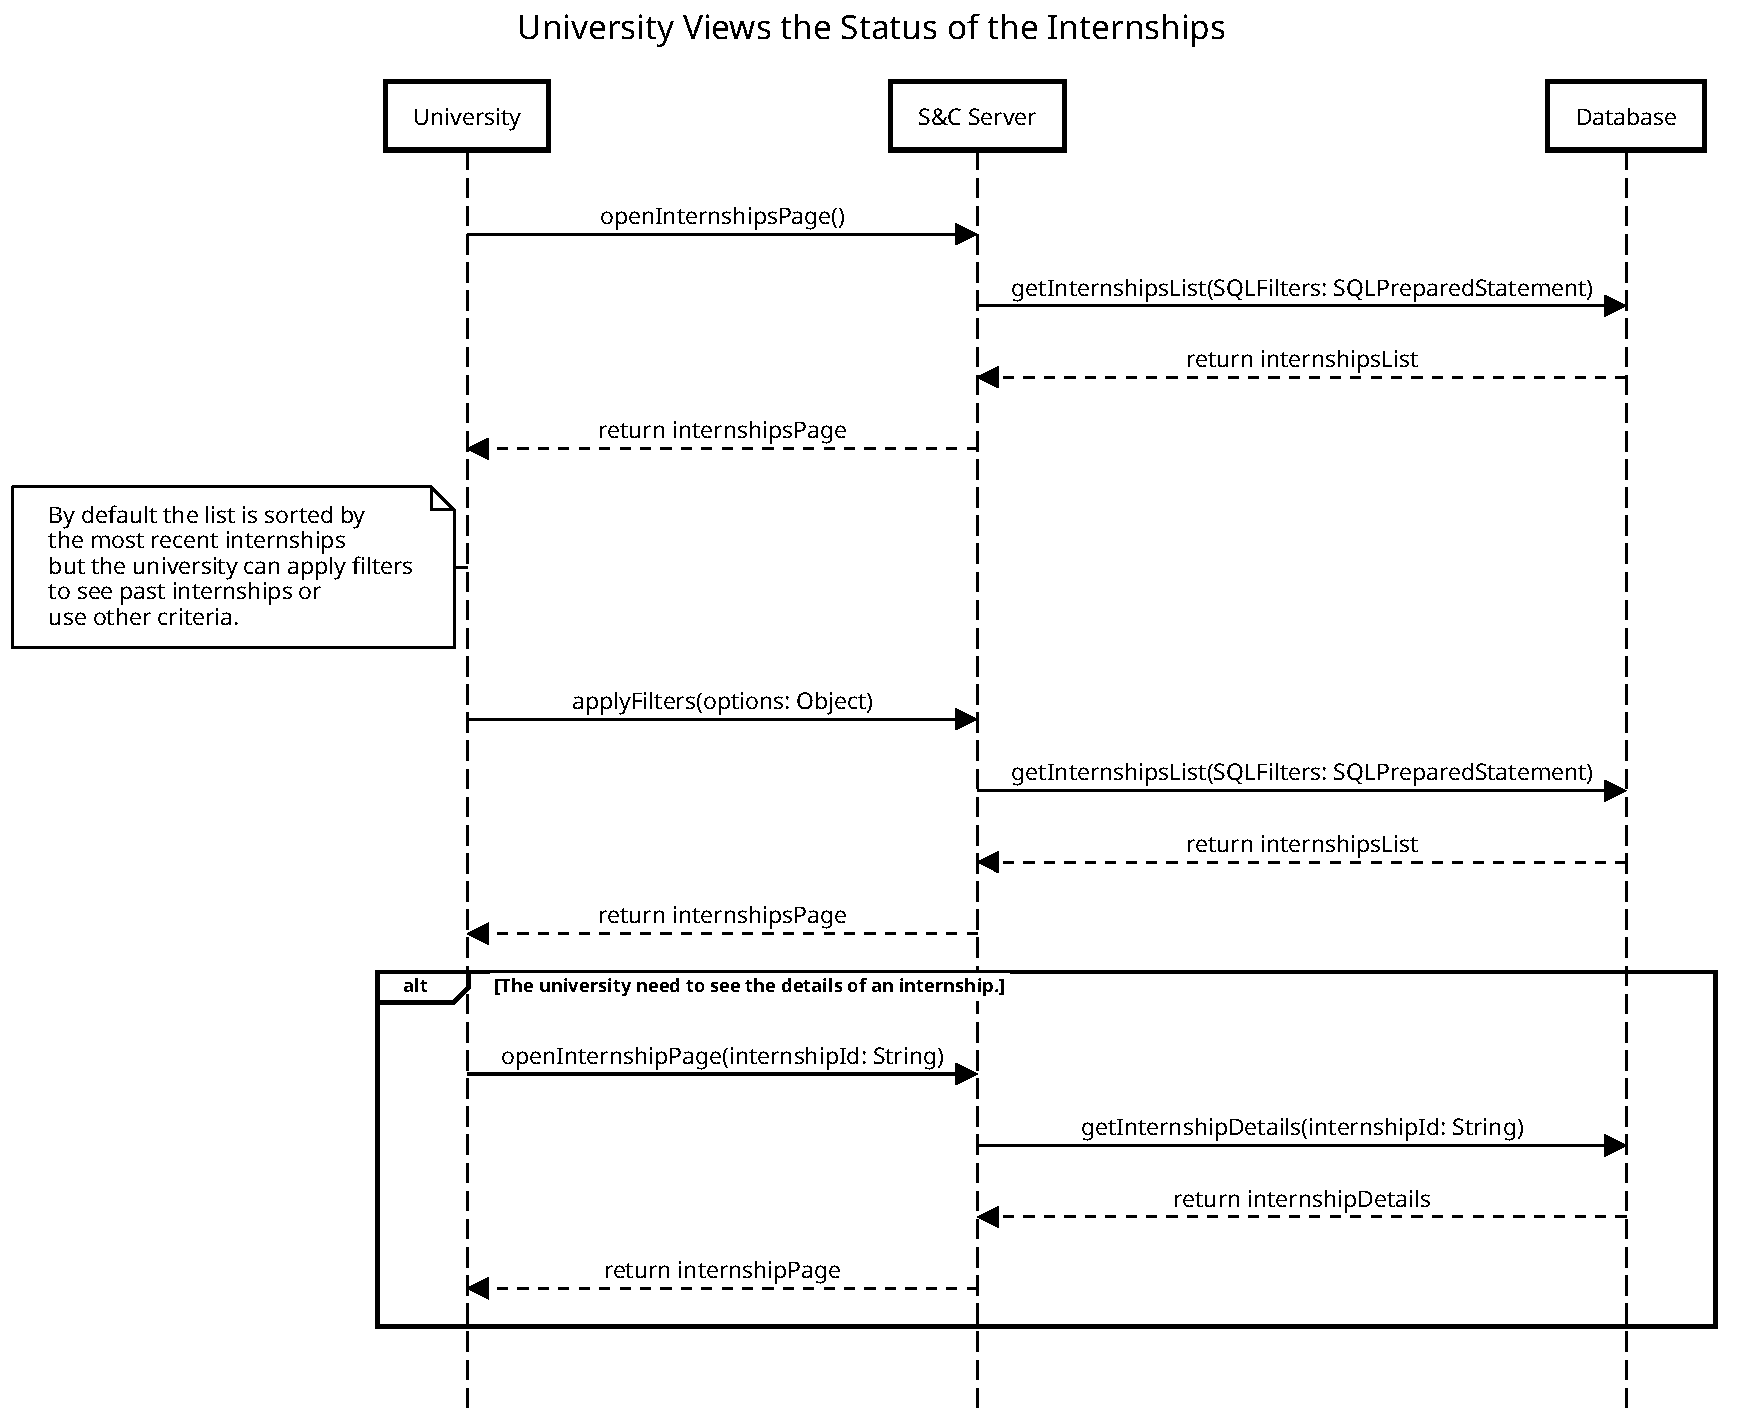
\includegraphics[width=1.0\textwidth]{Images/UC_15.pdf}
    \caption{University Views the Status of the Internships - Use Case Diagram}
    \label{fig:use-case-diagram-16}
\end{figure}

% 17

\subsubsection{UC17: University reviews and handles a complaint}
\label{subsubsec:university-reviews-and-handles-a-complaint}

\begin{center}
    \begin{longtable}{|l|p{0.75\linewidth}|}
        \hline
        \textbf{Actors:}           & UN                                                                                                    \\
        \hline
        \textbf{Entry Conditions:} & UN is correctly logged in. The UN has a list of complaints to review.                                 \\
        \hline
        \textbf{Flow of Events:}   & \begin{enumerate}
                                         \item UN clicks on the "Complaints" button.
                                         \item S\&C fetch the complaints from the database.
                                         \item S\&C shows a preview of the complaints to the UN.
                                         \item UN selects a complaint to review.
                                         \item S\&C fetch the complaint details from the database.
                                         \item S\&C shows the complaint details to the UN.
                                         \item UN review the complaint and writes a response and decide if the internship need to be suspended.
                                         \item S\&C update the status of the complaint with the UN response.
                                         \item S\&C suspend the internship if the UN decided to do so.
                                         \item S\&C notifies the UN that the complaint was successfully reviewed.
                                     \end{enumerate} \\
        \hline
        \textbf{Exit Conditions:}  & UN receive the confirmation of the complaint being reviewed correctly.                                \\
        \hline
        \textbf{Exceptions:}       & S\&C generated an internal error.                                                                     \\
        \hline
    \end{longtable}
\end{center}

\begin{figure}[H]
    \centering
    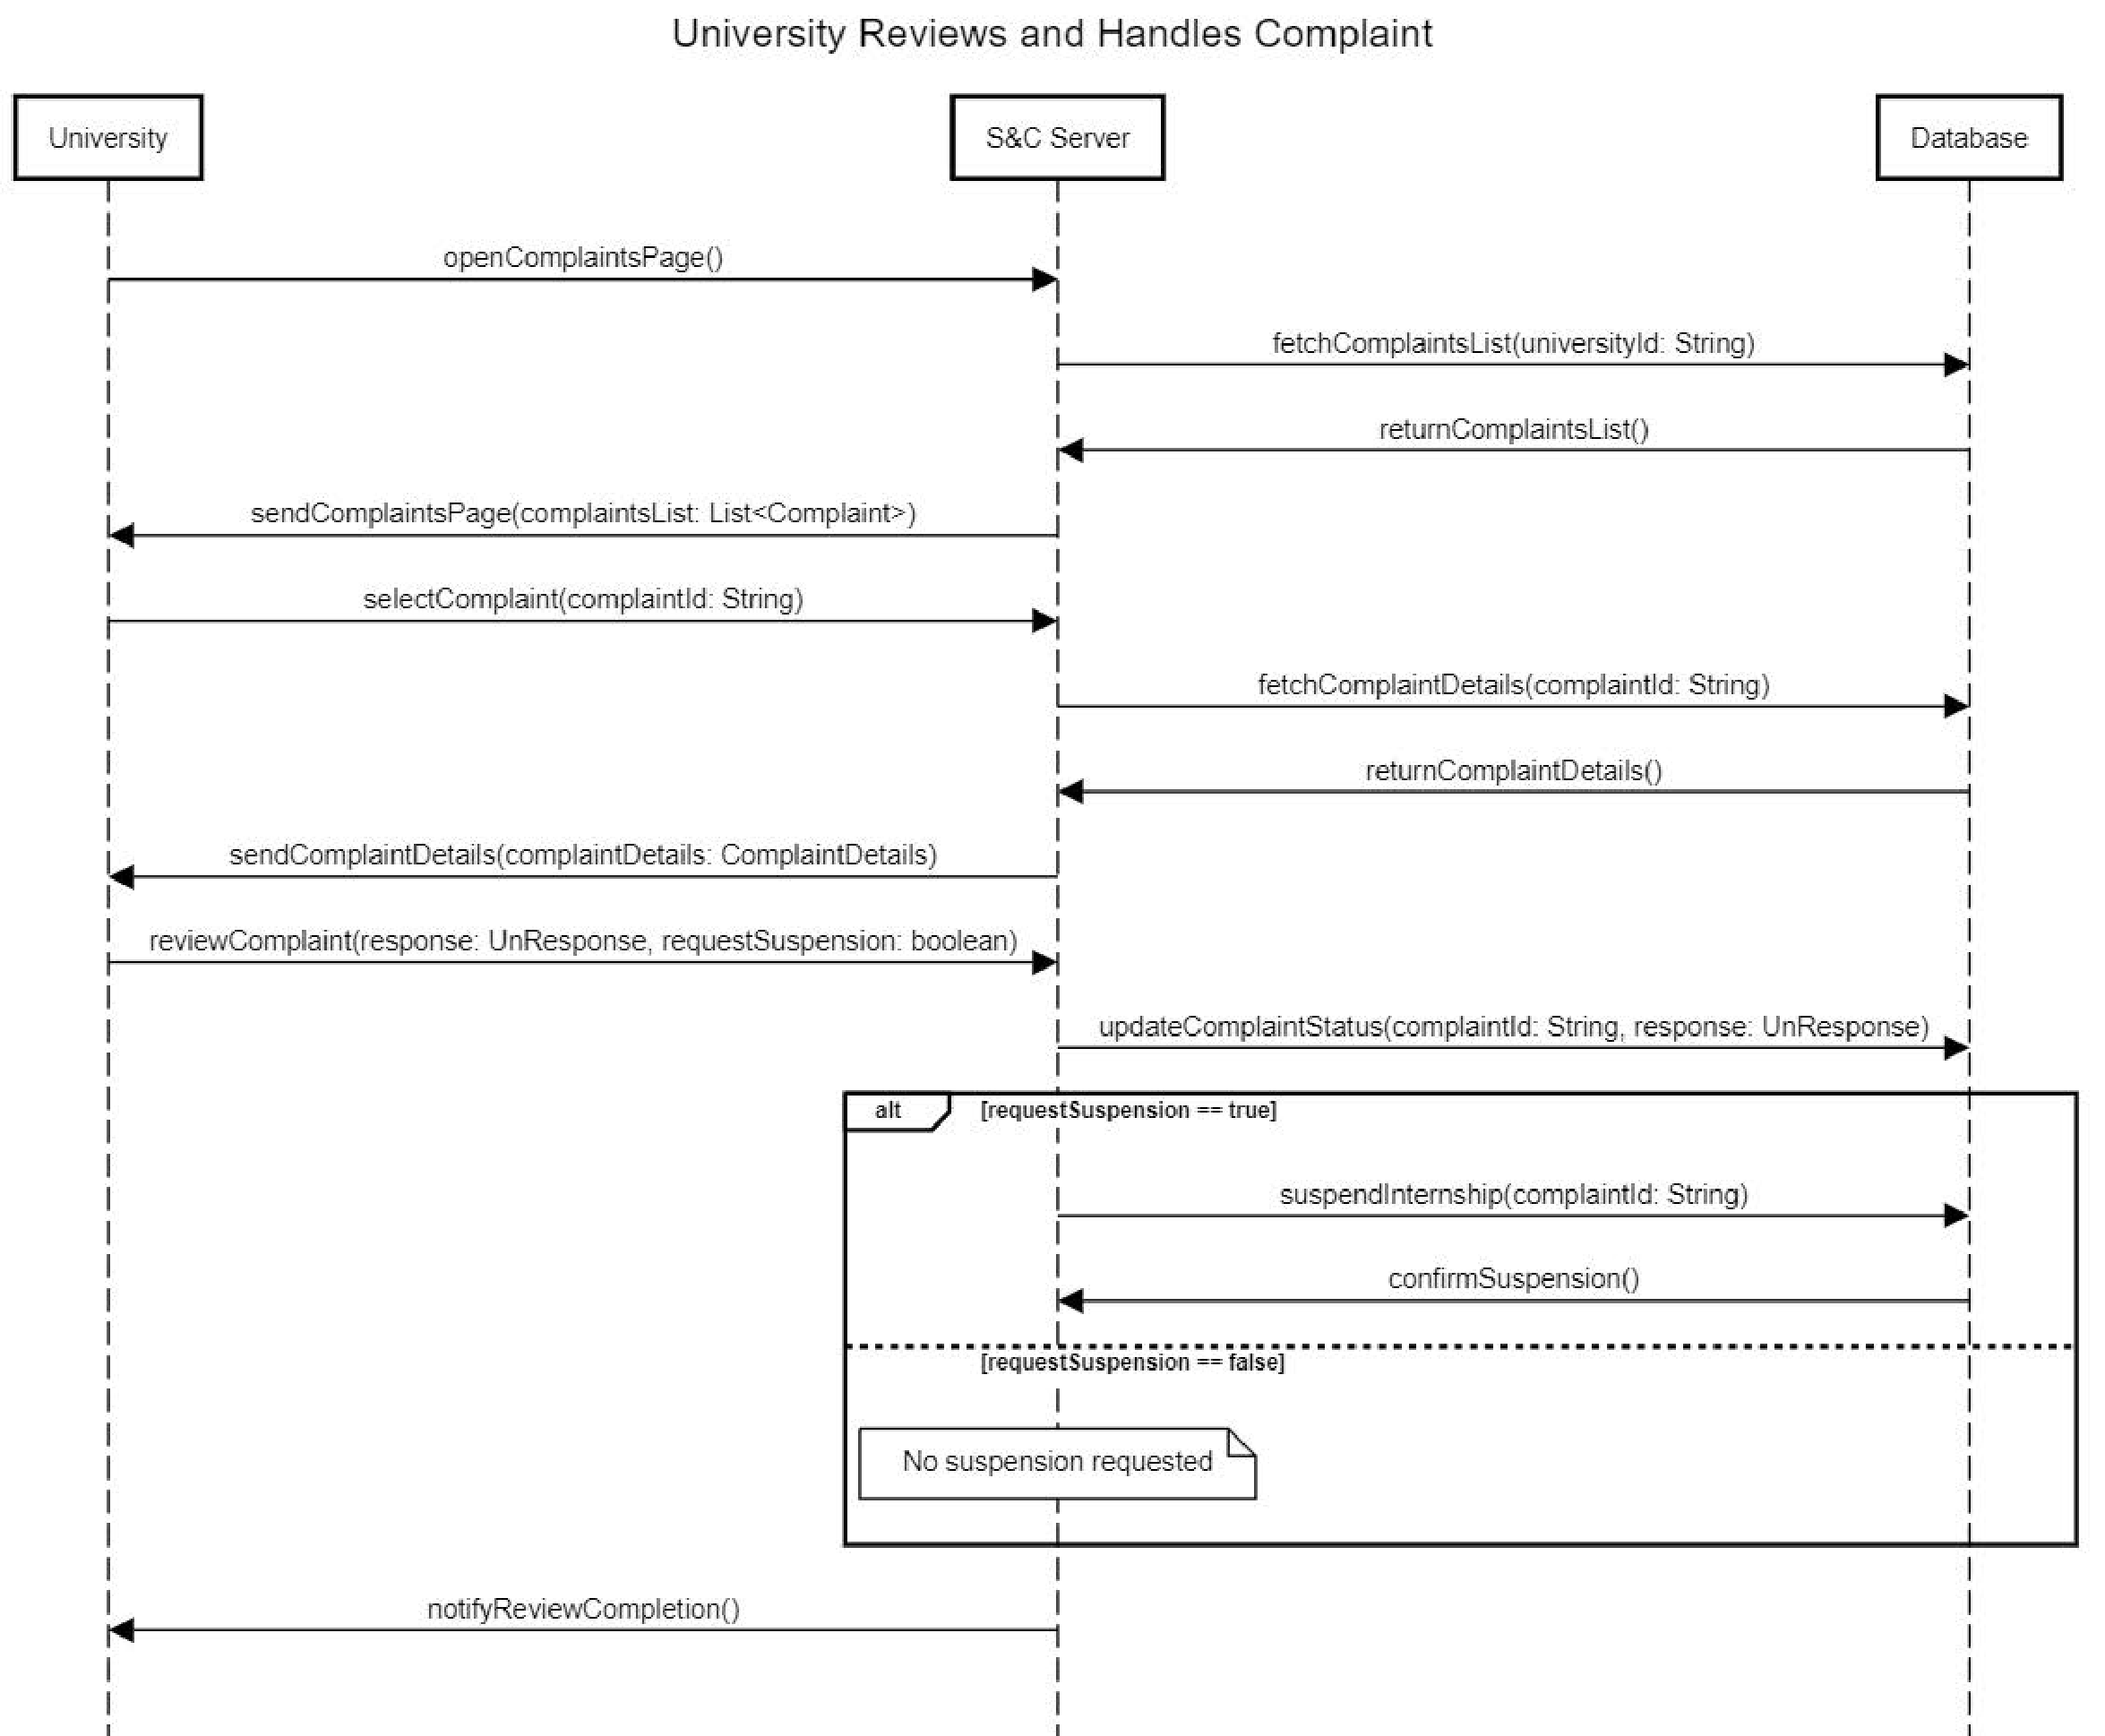
\includegraphics[width=1.0\textwidth]{Images/UC_16.pdf}
    \caption{University Reviews and Handles a Complaint - Use Case Diagram}
    \label{fig:use-case-diagram-17}
\end{figure}

% 18

\subsubsection{UC18: University blocks a malicious company}
\label{subsubsec:university-blocks-a-malicious-company}

\begin{center}
    \begin{longtable}{|l|p{0.75\linewidth}|}
        \hline
        \textbf{Actors:}           & UN                                                                                                            \\
        \hline
        \textbf{Entry Conditions:} & UN is correctly logged in and it has received a serious complaint that requires the blocks of a malicious CO. \\
        \hline
        \textbf{Flow of Events:}   & \begin{enumerate}
                                         \item UN visits the "My Contract" page.
                                         \item S\&C fetches the agreement between UN and corporate.
                                         \item S\&C shows the legal documents currently effective between UN and S\&C corp.
                                         \item UN clicks on "Block a Company" and enters the CO id (ex. P.IVA) of the malicious company.
                                         \item S\&C updates the UN's blacklist adding the specified CO.
                                         \item S\&C shows the user a confirmation.
                                     \end{enumerate}                \\
        \hline
        \textbf{Exit Conditions:}  & UN has now successfully "burnt all the bridges" between its STs and the affected CO.                          \\
        \hline
        \textbf{Exceptions:}       & S\&C generated an internal error. Invalid CO's identifier.                                                    \\
        \hline
    \end{longtable}
\end{center}

\begin{figure}[H]
    \centering
    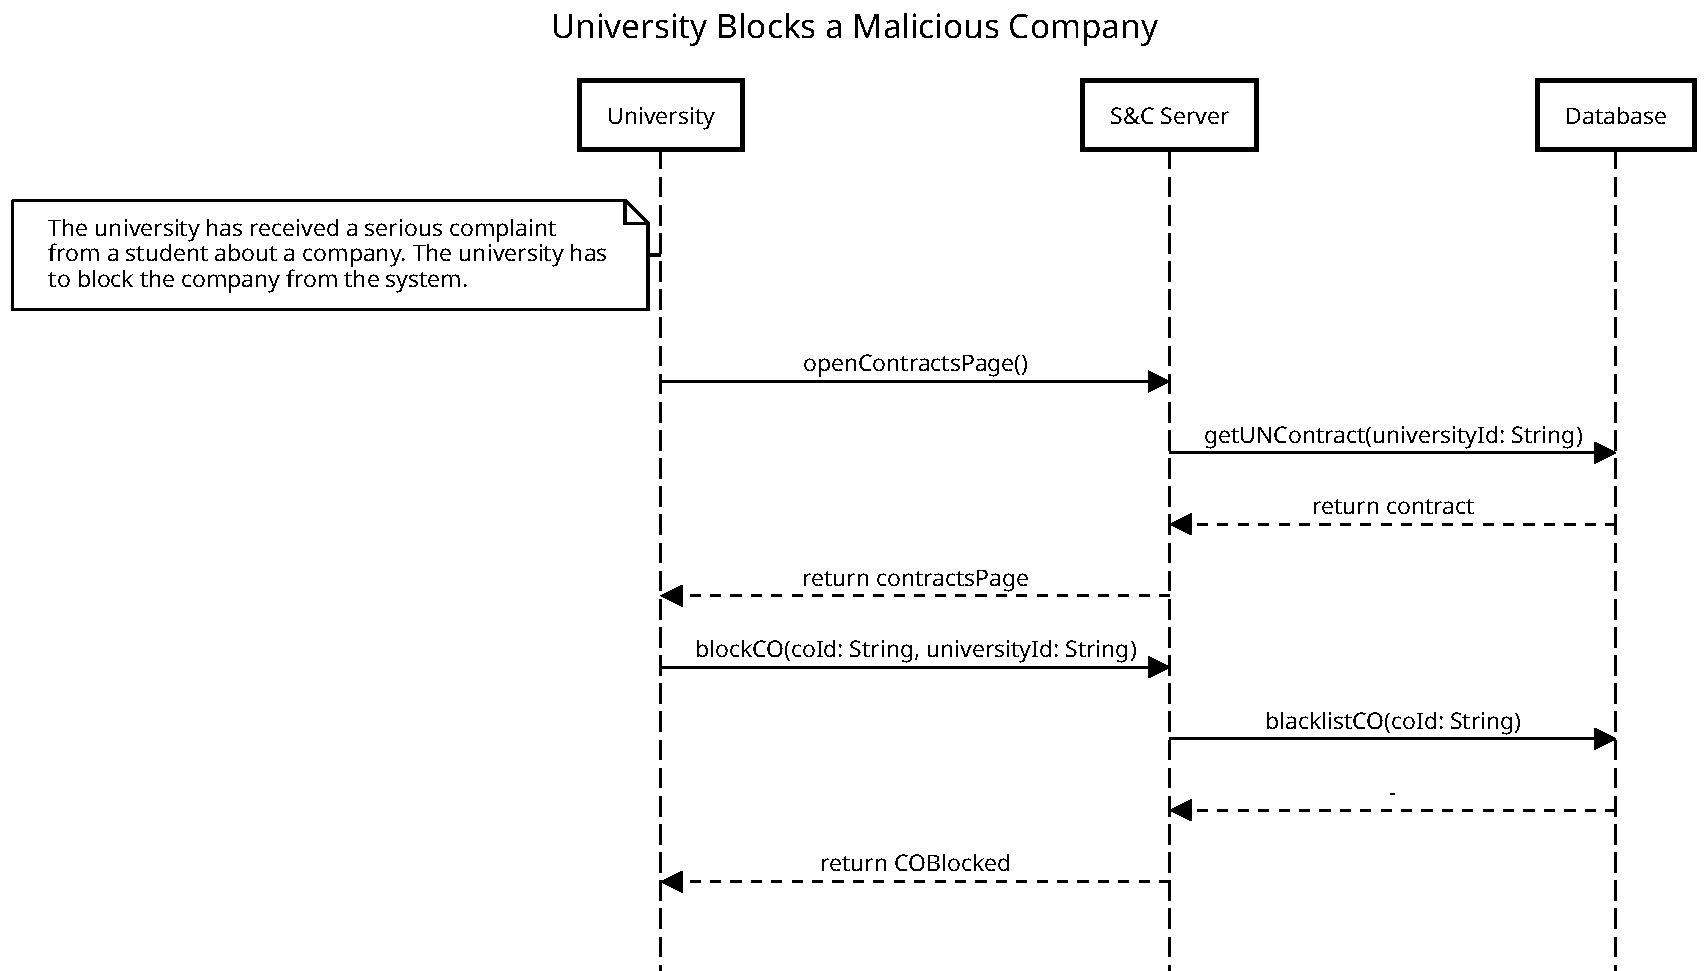
\includegraphics[width=1.0\textwidth]{Images/UC_17.pdf}
    \caption{University Blocks a Malicious Company - Use Case Diagram}
    \label{fig:use-case-diagram-18}
\end{figure}
